%%%%%%%%%%%%%%%%%%%%%%%%%%%%%%%%%%%%%%%%%%%%%%%%%%%%%%%%%%%%%%%%%%%%%%%%%%%
\section{Operating Systems for Embedded Systems}
%%%%%%%%%%%%%%%%%%%%%%%%%%%%%%%%%%%%%%%%%%%%%%%%%%%%%%%%%%%%%%%%%%%%%%%%%%%
\nsl{Advances in microcontroller technology continue to open up new application fields for embedded systems. In parallel with this trend,
the equipment controlled by embedded systems has become more sophisticated, often incorporating many functions in one product.
As a result, embedded systems have grown in scale and complexity. Moreover, as products increasingly adopt digital technology,
advanced processors have enabled more of the processing to be implemented in software, making embedded systems all the more important.
\newline
This means, in new application the developer is more and more interested to do the software development
with the support of an operating system. Especially in large scale systems the effect on reducing development cost with an operating system is important.
\newline
Even in the small-scale embedded system field, the growing scale and complexity of software and the need for fast
development turnaround time have made improving software productivity a pressing need. The use of C and other high-level languages
have become increasingly common for this reason.
\newline
Real time operating systems fulfil all the requirements from the developer. They guarantee a response of the system in specific time.
The development cycle becomes much shorter if the user could do the development on the target. Cross-development involves the downloading
of the executable program on the target, testing it, changing it and repeating the same procedure once more for the next error
is not an optimal development cycle. Real time operating systems offer a good support for the debugging.
\newline
There exist only a few drawbacks if you are looking for appropriate real time operating system. The first most important disadvantages
of the most real time operating systems are the costs. The second one is that real time operating systems need virtual memory system which is in
special not available in small microcontrollers.
\newline
The virtual memory system itself is really suitable for general purpose applications like a desktop PC.
But for embedded systems a virtual memory system makes the application more difficult. In such systems really often an access to the hardware
is necessary (control interfaces). These programming aspects could only be done in the so called ``kernel-mode'' with the result that such
programs more dangerous (collapse of the operating system) and more difficult to test.
\newline
In this chapter we will discuss some aspects of operating systems and than come to the uCLinux or other ``embedded Linux Systems'', operating systems
for microcontroller with and without a virtual memory system.
}
\bigskip
\bi
	\ite a lot of embedded systems runs without a operating system
	\bi
		\ite only  small algorithm (e.g. 'control the window' open/close system in a car).
		\ite hard restrictions in the size of memory especially by 8- and 16-bit microcontrollers.
		\ite costs of an operating system.
	\ei
	\bigskip
	\ite reasons for the use of an operating system
	\bi
		\ite generally the same reasons why we need one for a traditional computer.
		\ite but in the case of embedded systems not all services of an operating systems are needed for any device.
		\ite embedded systems have a large variety of requirements and environments.
		\bi
			\ite critical applications with high functionality (medical applications, aircraft systems ..).
			\ite critical applications with small functionality (ABS, cardiac pacemaker ..).
			\ite not very critical applications with varying functionality (mobile phone microwave ofen, washing machine ..).
		\ei

	\ei
\ei

\begin{description}
\item[{\rot\bf Special operating system (OS) for embedded systems}]~\\[-3ex]
\bigskip
\bi
	\ite a standard OS (like Windows or Linux) isn't suitable because :
	\bi
		\ite monolithic kernel has too many features which are not necessary in a specific application.
		\ite monolithic kernel is not modular, fault-tolerant, configurable, modifiable.
		\ite needs too much memory space (virtual memory).
		\ite not designed for mission-critical applications.	
	\ei
\ei
\bigskip
\item[{\rot\bf Key features of an OS for embedded systems }]~\\[-3ex]
\bigskip
\bi
	\ite configurability \pr no single OS will fit all needs, so configurability needed
	\bi
		\ite simplest form \pr remove unused functions (by linker ?)
		\ite conditional compilation (using \#if and \#ifdef commands)
		\ite dynamic data might be replaced by static data
		\ite removes unnecessary functions or modules by a kernel programming (Linux, eCos, VxWORKS).
	\ei
	\bigskip
	\ite handling of device drivers
	\bi
		\ite access to interfaces.
		\ite device drivers handled by tasks instead of integrated drivers.
		\ite improve predictability; everything goes through scheduler.
  		\ite in embedded systems mostly a lot of different interfaces are available, so not every device needs support by all versions of the OS.
	\ei
\ei

\begin{figure}[!hbtp]
     \begin{center}
	  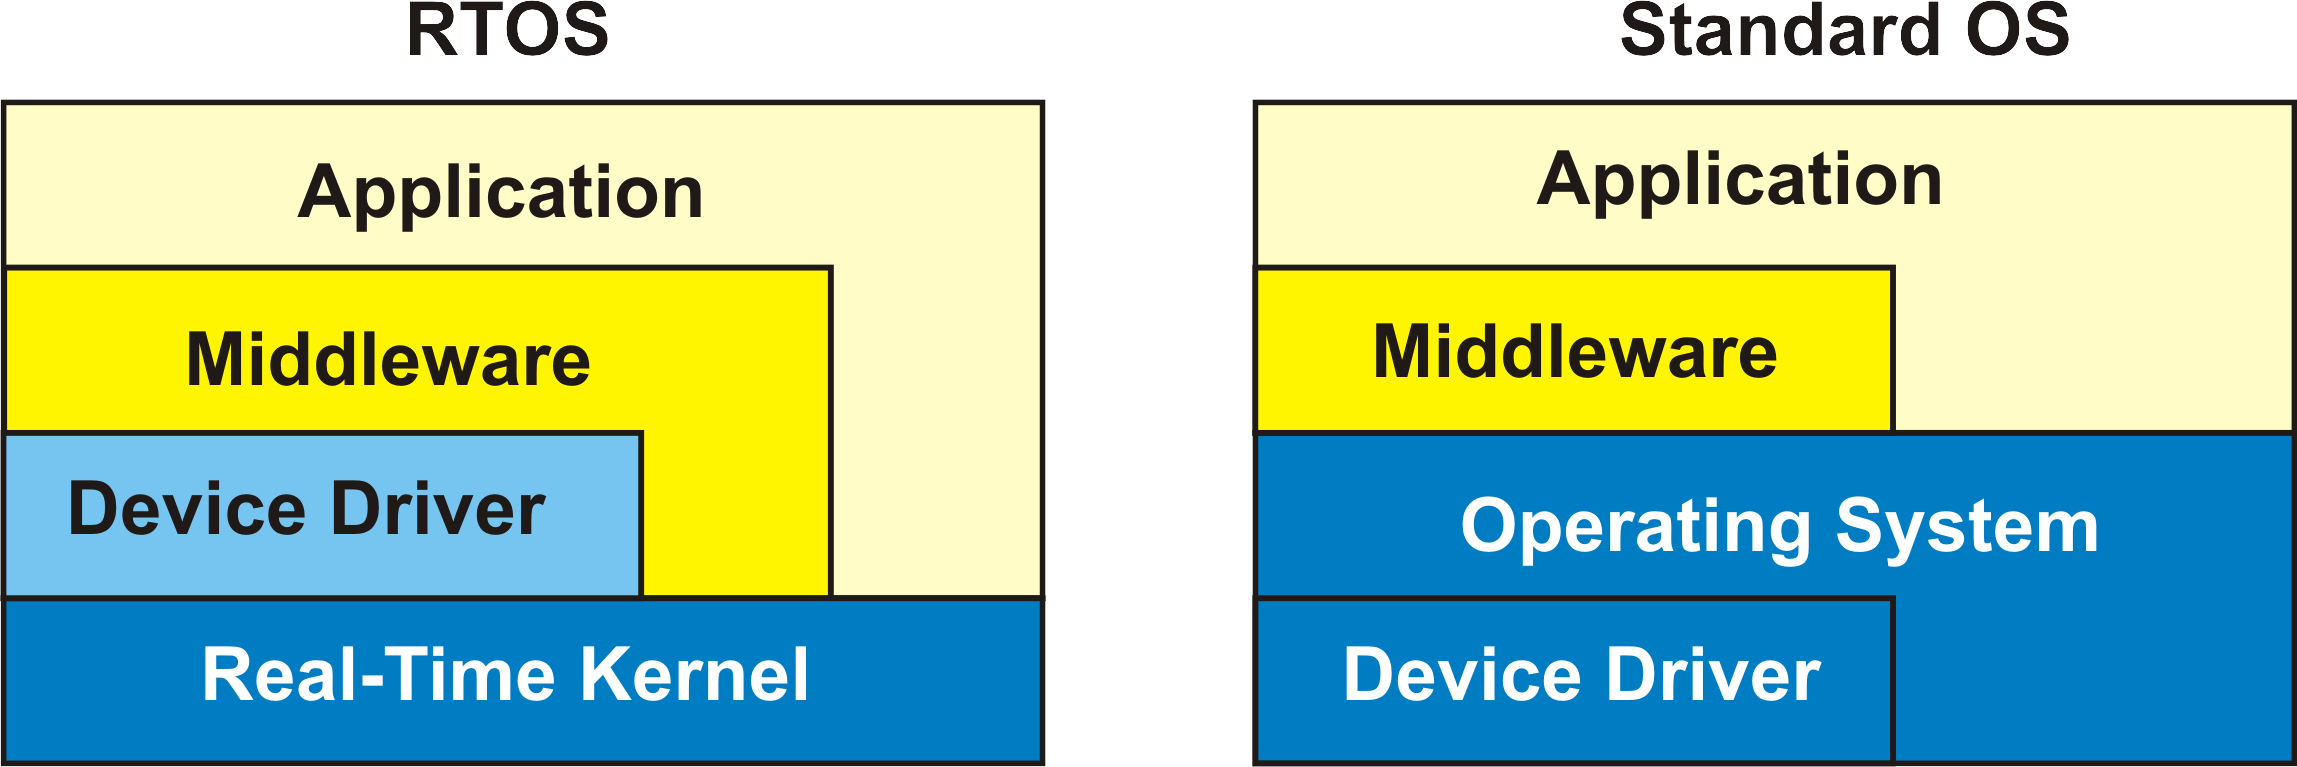
\epsfig{file=figures/Fig_6_1_RTOS_StandardOS,width=0.8\textwidth}\\
	  \caption{Integration of Devices Drivers in an OS}
     \end{center}
\end{figure}
\os{\newpage}

\bigskip
\bi
	\ite handling of interupts
	\bi
		\ite for standard OS: serious source of unreliability.
		\ite it should be possible to let interrupts directly start or stop tasks (by storing the tasks start address in the interrupt table).
	\ei
\ei

\item[{\rot\bf Available OS for embedded systems}]~\\[-3ex]
\bigskip
\bi
	\ite QNX
	\bi
		\ite real time operating system based on micro core technology.
		\ite suitable for small and large embedded systems.
		\ite tasks are separated in its one address space.
		\ite scheduling event driven (restrictions in time based scheduling) .
	\ei
	\bigskip
	\ite VxWORKS
	\bi
		\ite small VxWorks Kernel.
		\ite no virtual memory space (dangerous if a task is not cooperative).
		\ite scheduling time, priority and event driven.
		\ite implemented on a lot of microcontrollers.
	\ei
	\bigskip
	\ite OSEK/VDX
	\bi
		\ite scalable real time OS build for application in the automotive area.
		\ite event driven execution of tasks.
		\ite operates with fixed priorities.
		\ite tasks are grouped in basic tasks and extended tasks.
		\ite no virtual memory system.
	\ei
	\os{\newpage}
	\ite eCos
	\bi
		\ite open source system.
		\ite scalable system (the configuration allows the application writer to impose their requirements on the run-time component).
		\ite OS and application software are specific for an embedded system.
		\ite scheduling is time and event driven.
		\ite no virtual memory system.
	\ei
	\bigskip
	\ite embedded Linux
	\bi
		\ite open source system.
		\ite scalable and portable (especially for 32 bit microcontrollers).
		\ite run with a non virtual and a virtual memory system.
		\ite scheduling is time and priority driven.
		\ite with the RTAI (\underline{r}eal \underline{t}ime \underline{a}pplication \underline{i}nterface) also a event driven scheduling mechanismn possible.
		\ite for small and large embedded systems.
	\ei
\ei
\end{description}
\os{\newpage}

%%%%%%%%%%%%%%%%%%%%%%%%%%%%%%%%%%%%%%%%%%%%%%%%%%%%%%%%%%%%%%%%%%%%%%%%%%%
\section{Functions of RTOS}
%%%%%%%%%%%%%%%%%%%%%%%%%%%%%%%%%%%%%%%%%%%%%%%%%%%%%%%%%%%%%%%%%%%%%%%%%%%
\begin{description}


\item[{\rot\bf FreeRTOS}]~\\[-3ex]
\bi
\ite FreeRTOS is a real-time kernel/scheduler on top of which MCU applications can be built to meet their hard real-time requirements.
\bi
\ite Allows MCU applications be organized as a collection of independent threads of execution.
\ite Decides which thread should be executed by examining the priority assigned to each thread.
\bi
\ite Assume a single core MCU where only a single thread can be executing at one time.
\ei
\ei
\ei

\os{\newpage} \item[{\rot\bf The simplest case of task priority assignments}]~\\[-3ex]
\bi
\ite Assign higher priorities (lower priorities) to threads that implement hard real-time (soft real-time) requirements
\bi
\ite As a result hard real-time threads are always executed ahead of soft real-time threads.
\ei
\ite But priority assignment decision are not always that simple.
\ite In general task prioritization can help ensure an application meet its processing deadline.
\ei

\os{\newpage}



\item[{\rot\bf Why use a real-time kernel}]~\\[-3ex]
\bi
\ite For a simple system many well-established techniques can provide an  appropriate solution without the use of a kernel.
\ite For a more complex embedded application a kernel would be preferable.
\ite But where the crossover point occurs will always be subjective.
\ite Besides ensuring an application meets its processing deadline a kernel can bring other less obvious benefits.
\ei

\os{\newpage}



\item[{\rot\bf Benefits of using real-time kernel 1}]~\\[-3ex]
\bi
\ite Abstracting away timing information
\bi
\ite Kernel is responsible for execution timing and provides a time-related API to the application. This allows the application code to be simpler and the overall code size be smaller.
\ei
\ite Maintainability/Extensibility
\bi
\ite Abstracting away timing details results in fewer interdependencies between modules and allows sw to evolve in a predictable way.
\ite Application performance is less susceptible to changes in the underlying hardware.
\ei
\ite Modularity
\bi
\ite Tasks are independent modules each of which has a well-defined purpose.
\ei
\ite Team development
\bi
\ite Tasks have well-defined interfaces allowing easier development by teams
\ei
\ei

\os{\newpage}



\item[{\rot\bf Benefits of using real-time kernel 2}]~\\[-3ex]
\bi
\ite Easier testing
\bi
\ite Tasks are independent modules with clean interfaces they can be tested in isolation.
\ei
\ite Idle time utilization
\bi
\ite The idle task is created automatically when the kernel is started. It executes whenever there are no application tasks to run.
\ite Be used to measure spare processing capacity perform background checks or simply place the process into a low-power mode.
\ei
\ite Flexible interrupt handling
\bi
\ite Interrupt handlers can be kept very short by deferring most of the required processing to handler tasks.
\ei
\ei

\os{\newpage}



\item[{\rot\bf Standard FreeRTOS features}]~\\[-3ex]
\bi
\ite Pre-emptive or co-operative operation
\ite Very flexible task priority assignment
\ite Queues
\ite Binary/Counting / Recursive semaphores
\ite Mutexes
\ite Tick/Idle hook functions
\ite Stack overflow checking
\ite Trace hook macros
\ite Interrupt nesting
\ei

\os{\newpage}


\item[{\rot \bf FreeRTOS - RT and Embedded}]~\\[-3ex]
\bi
\ite "Embedded" and "real-time" can mean different things to different people, so let's define them as FreeRTOS uses them.
\ite An embedded system is a computer system that is designed to do only a few things, like the system in a TV remote control, in-car GPS, digital watch, or pacemaker. Embedded systems are typically smaller and slower than general purpose computer systems, and are also usually less expensive. A typical low-end embedded system may have an 8-bit CPU running at 25MHz, a few KB of RAM, and maybe 32KB of flash memory. A higher-end embedded system may have a 32-bit CPU running at 750MHz, a GB of RAM, and multiple GB of flash memory.
\ite Real-time systems are designed to do something within a certain amount of time; they guarantee that stuff happens when it's supposed to.
\ite A pacemaker is an excellent example of a real-time embedded system. A pacemaker must contract the heart muscle at the right time to keep you alive; it can't be too busy to respond in time. Pacemakers and other real-time embedded systems are carefully designed to run their tasks on time, every time.
\ei

\os{\newpage}



\item[{\rot\bf Architecture}]~\\[-3ex]
\bi
\ite FreeRTOS is a relatively small application. The minimum core of FreeRTOS is only three source (.c) files and a handful of header files, totalling just under 9000 lines of code, including comments and blank lines. A typical binary code image is less than 10KB.

\ite FreeRTOS's code breaks down into three main areas: tasks, communication, and hardware interfacing.

\ite Tasks: Almost half of FreeRTOS's core code deals with the central concern in many operating systems: tasks. A task is a user-defined C function with a given priority. tasks.c and task.h do all the heavy lifting for creating, scheduling, and maintaining tasks.

\ite Communication: Tasks are good, but tasks that can communicate with each other are even better! Which brings us to the second FreeRTOS job: communication. About 40\% of FreeRTOS's core code deals with communication. queue.c and queue.h handle FreeRTOS communication. Tasks and interrupts use queues to send data to each other and to signal the use of critical resources using semaphores and mutexes.

\ite The Hardware Whisperer: The approximately 9000 lines of code that make up the base of FreeRTOS are hardware-independent; the same code runs whether FreeRTOS is running on the humble 8051 or the newest, shiniest ARM core. About 6\% of FreeRTOS's core code acts a shim between the hardware-independent FreeRTOS core and the hardware-dependent code. We'll discuss the hardware-dependent code in the next section.
\ei

\os{\newpage}



\item[{\rot\bf Hardware Considerations}]~\\[-3ex]
\bi
\ite The hardware-independent FreeRTOS layer sits on top of a hardware-dependent layer. This hardware-dependent layer knows how to talk to whatever chip architecture you choose.
\ei
\begin{figure}[!hbtp]
     \begin{center}
	  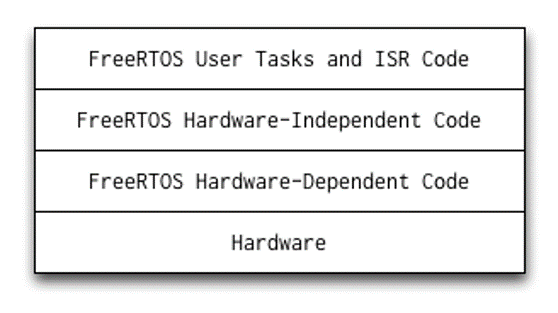
\epsfig{file=figures/Fig_6_1_00rtos.png,width=0.8\textwidth}\\
	  \caption{FreeRTOS Layers}
     \end{center}
\end{figure}

\os{\newpage}


\item[{\rot\bf Configurations}]~\\[-3ex]
\bi
\ite Configuration options are selected in FreeRTOSConfig.h by setting various \#defines. Clock speed, heap size, mutexes, and API subsets are all configurable in this file, along with many other options. Here are a few examples that set the maximum number of task priority levels, the CPU frequency, the system tick frequency, the minimal stack size and the total heap size:

\begin{lstlisting}[language=C]
#define configMax\_PRIORITIES     (( unsigned portBASE\_TYPE)5)
#define configCPU_CLOCK_HZ        (12000000UL)
#define configTICK_RATE_HZ        (( portTickType ) 1000)
#define configMINIMAL_STACK_SIZE  (( unsigned short ) 100)
#define configTOTAL\_HEAP\_SIZE   (( size_t ) ( 4 * 1024 ))
\end{lstlisting}
\ei

\os{\newpage}



\item[{\rot\bf Hardware Dependency}]~\\[-3ex]
\bi
\ite Hardware-dependent code lives in separate files for each compiler toolchain and CPU architecture.
\ite For example, if you're working with the IAR compiler on an ARM Cortex-M3 chip, the hardware-dependent code lives in the FreeRTOS/Source/portable/IAR/ARM\_CM3/ directory.
\ite portmacro.h declares all of the hardware-specific functions, while port.c and portasm.s contain all of the actual hardware-dependent code.
\ite The hardware-independent header file portable.h \#include's the correct portmacro.h file at compile time. FreeRTOS calls the hardware-specific functions using \#define'd functions declared in portmacro.h.
\ei

\os{\newpage}



\item[{\rot\bf Example}]~\\[-3ex]
\bi
\ite Let's look at an example of how FreeRTOS calls a hardware-dependent function. The hardware-independent file tasks.c frequently needs to enter a critical section of code to prevent preemption. Entering a critical section happens differently on different architectures, and the hardware-independent tasks.c does not want to have to understand the hardware-dependent details.
\ite So tasks.c calls the global macro portENTER\_CRITICAL(), glad to be ignorant of how it actually works.
\ite Assuming we're using the IAR compiler on an ARM Cortex-M3 chip, FreeRTOS is built with the file
\ite  FreeRTOS/Source/portable/IAR/ARM\_CM3/portmacro.h which defines portENTER\_CRITICAL() like this:
\ite \#define portENTER\_CRITICAL()   vPortEnterCritical()
\ei

\os{\newpage}



\item[{\rot\bf Example 2}]~\\[-3ex]
\bi
\ite vPortEnterCritical() is actually defined in
\bi
\ite FreeRTOS/Source/portable/IAR/ARM\_CM3/port.c.
\ite The port.c file is hardware-dependent, and contains code that understands the IAR compiler and the Cortex-M3 chip.
\ite vPortEnterCritical() enters the critical section using this hardware-specific knowledge and returns to the hardware-independent tasks.c.
\ei
\ite The portmacro.h file also defines an architecture's basic data types. Data types for basic integer variables, pointers, and the system timer tick data type are defined like this for the IAR compiler on ARM Cortex-M3 chips:
\begin{lstlisting}[language=C]
\ite #define portBASE\_TYPE  long              // Basic integer variable type
\ite #define portSTACK_TYPE unsigned long     // Pointers to memory locations
\ite typedef unsigned portLONG portTickType;  // The system timer tick type
\end{lstlisting}
\ei

\os{\newpage}



\item[{\rot\bf Example 3}]~\\[-3ex]
\bi
\ite This method of using data types and functions through thin layers of \#defines may seem a bit complicated, but it allows FreeRTOS to be recompiled for a completely different system architecture by changing only the hardware-dependent files. And if you want to run FreeRTOS on an architecture it doesn't currently support, you only have to implement the hardware-dependent functionality which is much smaller than the hardware-independent part of FreeRTOS.
\ite As we've seen, FreeRTOS implements hardware-dependent functionality with C preprocessor \#define macros. FreeRTOS also uses \#define for plenty of hardware-independent code. For non-embedded applications this frequent use of \#define is a cardinal sin, but in many smaller embedded systems the overhead for calling a function is not worth the advantages that "real" functions offer.
\ei

\os{\newpage}



\item[{\rot\bf Full task state machine}]~\\[-3ex]
\begin{center}
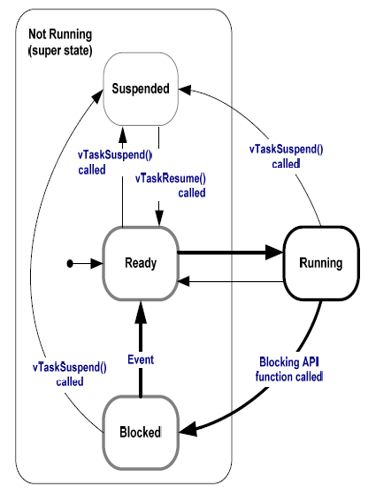
\includegraphics[height=12 cm]{figures/Fig_6_1_07rtos.png}
\end{center}

\os{\newpage}



{\rot \bf Tasks - Task Control Block in tasks.c}

\begin{lstlisting}[language=C]

typedef struct tskTaskControlBlock
{
   volatile portSTACK_TYPE *pxTopOfStack;      /* Points to the location of the last item placed on the tasks stack.  THIS MUST BE THE FIRST MEMBER OF THE STRUCT. */

   xListItem    xGenericListItem;                          /* List item used to place
                                                              the TCB in ready and
                                                              blocked queues. */
   xListItem    xEventListItem;                            /* List item used to place
                                                              the TCB in event lists.*/
   unsigned portBASE\_TYPE uxPriority;                      /* The priority of the task
                                                              where 0 is the lowest
                                                              priority. */
   portSTACK_TYPE *pxStack;                                /* Points to the start of
                                                              the stack. */
   signed char    pcTaskName[ configMAX_TASK\_NAME_LEN ];   /* Descriptive name given
                                                              to the task when created.
                                                              Facilitates debugging
                                                              only. */

   #if ( portSTACK_GROWTH > 0 )
     portSTACK_TYPE *pxEndOfStack;                         /* Used for stack overflow
                                                              checking on architectures
                                                              where the stack grows up
                                                              from low memory. */
   #endif

   #if ( configUSE_MUTEXES == 1 )
     unsigned portBASE\_TYPE uxBasePriority;                /* The priority last
                                                              assigned to the task -
                                                              used by the priority
                                                              inheritance mechanism. */
   #endif

 } tskTCB;

\end{lstlisting}


\os{\newpage}


\item[{\rot \bf Scheduling Tasks - Priorities and Ready List}]~\\[-3ex]
\bi
\ite Each task has a user-assigned priority between 0 (the lowest priority) and the compile-time value of configMAX\_PRIORITIES-1 (the highest priority). For instance, if configMAX\_PRIORITIES is set to 5, then FreeRTOS will use 5 priority levels: 0 (lowest priority), 1, 2, 3, and 4 (highest priority).

\ite FreeRTOS uses a "ready list" to keep track of all tasks that are currently ready to run. It implements the ready list as an array of task lists like this:
\ei

\begin{lstlisting}[language=C]
static xList pxReadyTasksLists[ configMax\_PRIORITIES ];  /* Prioritised ready tasks.  */
pxReadyTasksLists[0] is a list of all ready priority 0 tasks,
pxReadyTasksLists[1] is a list of all ready priority 1 tasks, and so on, all the way up to pxReadyTasksLists[configMax\_PRIORITIES-1].
\end{lstlisting}

\os{\newpage}



\item[{\rot\bf Scheduling Tasks - System Tick}]~\\[-3ex]

\bi
\ite The heartbeat of a FreeRTOS system is called the system tick. FreeRTOS configures the system to generate a periodic tick interrupt. The user can configure the tick interrupt frequency, which is typically in the millisecond range. Every time the tick interrupt fires, the vTaskSwitchContext() function is called. vTaskSwitchContext() selects the highest-priority ready task and puts it in the pxCurrentTCB variable like this:
\begin{lstlisting}[language=C]
 /* Find the highest-priority queue that contains ready tasks. */
 while( listLIST_IS_EMPTY( \&( pxReadyTasksLists[ uxTopReadyPriority ] ) ) )
 {
     configASSERT( uxTopReadyPriority );
     --uxTopReadyPriority;
 }

 /* listGET_OWNER_OF_NEXT_ENTRY walks through the list, so the tasks of the same
 priority get an equal share of the processor time. */
 listGET_OWNER_OF_NEXT_ENTRY( pxCurrentTCB, \&( pxReadyTasksLists[ uxTopReadyPriority ] ) );
\end{lstlisting}
\ei

\os{\newpage}



\item[{\rot\bf Scheduling Tasks - Ready List}]~\\[-3ex]
\bi
\ite Before the while loop starts, uxTopReadyPriority is guaranteed to be greater than or equal to the priority of the highest-priority ready task. The while() loop starts at priority level uxTopReadyPriority and walks down through the pxReadyTasksLists array to find the highest-priority level with ready tasks. listGET\_OWNER\_OF\_NEXT\_ENTRY() then grabs the next ready task from that priority level's ready list.

\ite Now pxCurrentTCB points to the highest-priority task, and when vTaskSwitchContext() returns the hardware-dependent code starts running that task.
\ite Those nine lines of code are the absolute heart of FreeRTOS. The other 8900+ lines of FreeRTOS are there to make sure those nine lines are all that's needed to keep the highest-priority task running.
\ei

\os{\newpage}




\nsl{

{\rot\bf Tasks - TCB}
\bi
\ite The TCB stores the address of the stack start address in pxStack and the current top of stack in pxTopOfStack. It also stores a pointer to the end of the stack in pxEndOfStack to check for stack overflow if the stack grows "up" to higher addresses. If the stack grows "down" to lower addresses then stack overflow is checked by comparing the current top of stack against the start of stack memory in pxStack.
\ite The TCB stores the initial priority of the task in uxPriority and uxBasePriority. A task is given a priority when it is created, and a task's priority can be changed. If FreeRTOS implements priority inheritance then it uses uxBasePriority to remember the original priority while the task is temporarily elevated to the "inherited" priority. (See the discussion about mutexes below for more on priority inheritance.)
\ite Each task has two list items for use in FreeRTOS's various scheduling lists. When a task is inserted into a list FreeRTOS doesn't insert a pointer directly to the TCB. Instead, it inserts a pointer to either the TCB's xGenericListItem or xEventListItem. These xListItem variables let the FreeRTOS lists be smarter than if they merely held a pointer to the TCB. We'll see an example of this when we discuss lists later.
\ite A task can be in one of four states: running, ready to run, suspended, or blocked. You might expect each task to have a variable that tells FreeRTOS what state it's in, but it doesn't. Instead, FreeRTOS tracks task state implicitly by putting tasks in the appropriate list: ready list, suspended list, etc. The presence of a task in a particular list indicates the task's state. As a task changes from one state to another, FreeRTOS simply moves it from one list to another.
\ei
}

\os{\newpage}



\item[{\rot\bf Tasks Setup}]~\\[-3ex]
\bi
\ite We've already touched on how a task is selected and scheduled with the pxReadyTasksLists array; now let's look at how a task is initially created. A task is created when the xTaskCreate() function is called. FreeRTOS uses a newly allocated TCB object to store the name, priority, and other details for a task, then allocates the amount of stack the user requests (assuming there's enough memory available) and remembers the start of the stack memory in TCB's pxStack member.
\ite The stack is initialized to look as if the new task is already running and was interrupted by a context switch. This way the scheduler can treat newly created tasks exactly the same way as it treats tasks that have been running for a while; the scheduler doesn't need any special case code for handling new tasks.
\ite The way that a task's stack is made to look like it was interrupted by a context switch depends on the architecture FreeRTOS is running on, but this ARM Cortex-M3 processor's implementation is a good example:
\ei

\os{\newpage}



\item[{\rot\bf Tasks - Stack}]~\\[-3ex]
\begin{lstlisting}[language=C]
 unsigned int *pxPortInitialiseStack( unsigned int *pxTopOfStack,
                                      pdTASK\_CODE pxCode,
                                      void *pvParameters )
 {
   /* Simulate the stack frame as it would be created by a context switch interrupt. */
   pxTopOfStack--; /* Offset added to account for the way the MCU uses the stack on
                      entry/exit of interrupts. */
   *pxTopOfStack = portINITIAL_XPSR;  /* xPSR */
   pxTopOfStack--;
   *pxTopOfStack = ( portSTACK_TYPE ) pxCode;  /* PC */
   pxTopOfStack--;
   *pxTopOfStack = 0;  /* LR */
   pxTopOfStack -= 5;  /* R12, R3, R2 and R1. */
   *pxTopOfStack = ( portSTACK_TYPE ) pvParameters;  /* R0 */
   pxTopOfStack -= 8;  /* R11, R10, R9, R8, R7, R6, R5 and R4. */

   return pxTopOfStack;
 }
\end{lstlisting}

\os{\newpage}



\item[{\rot\bf Tasks - Stack}]~\\[-3ex]
\bi
\ite The ARM Cortex-M3 processor pushes registers on the stack when a task is interrupted. pxPortInitialiseStack() modifies the stack to look like the registers were pushed even though the task hasn't actually started running yet. Known values are stored to the stack for the ARM registers xPSR, PC, LR, and R0. The remaining registers R1 -- R12 get stack space allocated for them by decrementing the top of stack pointer, but no specific data is stored in the stack for those registers. The ARM architecture says that those registers are undefined at reset, so a (non-buggy) program will not rely on a known value.
\ite After the stack is prepared, the task is almost ready to run. First though, FreeRTOS disables interrupts: We're about to start mucking with the ready lists and other scheduler structures and we don't want anyone else changing them underneath us.
\ite If this is the first task to ever be created, FreeRTOS initializes the scheduler's task lists. FreeRTOS's scheduler has an array of ready lists, pxReadyTasksLists, which has one ready list for each possible priority level. FreeRTOS also has a few other lists for tracking tasks that have been suspended, killed, and delayed. These are all initialized now as well.
\ite After any first-time initialization is done, the new task is added to the ready list at its specified priority level. Interrupts are re-enabled and new task creation is complete.
\ei

\os{\newpage}




\item[{\rot\bf Lists}]~\\[-3ex]
\bi
\ite The FreeRTOS list is a standard circular doubly linked list with a couple of interesting additions. Here's a list element:
\begin{lstlisting}[language=C]
 struct xLIST_ITEM
 {
   portTickType xItemValue;              /* The value being listed.  In most cases used to sort the list in descending order. */
   volatile struct xLIST_ITEM * pxNext;  /* Pointer to the next xListItem in the list.  */
   volatile struct xLIST_ITEM * pxPrevious;/* Pointer to the previous xListItem in the list. */
   void * pvOwner;                       /* Pointer to the object (normally a TCB) that contains the list item.  There is therefore a two-way link between the object containing the list item and the list item itself. */
   void * pvContainer;                   /* Pointer to the list in which this list item is placed (if any). */
 };
\end{lstlisting}
\ei

\os{\newpage}



\item[{\rot\bf Lists}]~\\[-3ex]
\bi
\ite Each list element holds a number, xItemValue, that is the usually the priority of the task being tracked or a timer value for event scheduling. Lists are kept in high-to-low priority order, meaning that the highest-priority xItemValue (the largest number) is at the front of the list and the lowest priority xItemValue (the smallest number) is at the end of the list.
\ite The pxNext and pxPrevious pointers are standard linked list pointers. pvOwner is a pointer to the owner of the list element. This is usually a pointer to a task's TCB object. pvOwner is used to make task switching fast in vTaskSwitchContext(): once the highest-priority task's list element is found in pxReadyTasksLists, that list element's pvOwner pointer leads us directly to the TCB needed to schedule the task.
\ite pvContainer points to the list that this item is in. It is used to quickly determine if a list item is in a particular list. Each list element can be put in a list, which is defined as:
\begin{lstlisting}[language=C]
 typedef struct xLIST
 {
   volatile unsigned portBASE\_TYPE uxNumberOfItems;
   volatile xListItem * pxIndex;           /* Used to walk through the list.  Points to
                                              the last item returned by a call to
                                              pvListGetOwnerOfNextEntry (). */
   volatile xMiniListItem xListEnd;        /* List item that contains the maximum
                                              possible item value, meaning it is always
                                              at the end of the list and is therefore
                                              used as a marker. */
 } xList;
\end{lstlisting}
\ei

\os{\newpage}



\item[{\rot\bf Lists}]~\\[-3ex]
\bi
\ite The size of a list at any time is stored in uxNumberOfItems, for fast list-size operations. All new lists are initialized to contain a single element: the xListEnd element. xListEnd.xItemValue is a sentinel value which is equal to the largest value for the xItemValue variable: 0xffff when portTickType is a 16-bit value and 0xffffffff when portTickType is a 32-bit value. Other list elements may also have the same value; the insertion algorithm ensures that xListEnd is always the last item in the list.
\ite Since lists are sorted high-to-low, the xListEnd element is used as a marker for the start of the list. And since the list is circular, this xListEnd element is also a marker for the end of the list.
\ite Most "traditional" list accesses you've used probably do all of their work within a single for() loop or function call like this:

\ei

\os{\newpage}

\item[{\rot\bf Lists}]~\\[-3ex]
\bi
\begin{lstlisting}[language=C]
for (listPtr = listStart; listPtr != NULL; listPtr = listPtr->next) {
   // Do something with listPtr here...
}
\end{lstlisting}
\ite FreeRTOS frequently needs to access a list across multiple for() and while() loops as well as function calls, and so it uses list functions that manipulate the pxIndex pointer to walk the list. The list function listGET\_OWNER\_OF\_NEXT\_ENTRY() does pxIndex = pxIndex->pxNext; and returns pxIndex. (Of course it does the proper end-of-list-wraparound detection too.) This way the list itself is responsible for keeping track of "where you are" while walking it using pxIndex, allowing the rest of FreeRTOS to not worry about it.
\ei

\os{\newpage}




\item[{\rot\bf Lists}]~\\[-3ex]
\bi
\ite The pxReadyTasksLists list manipulation done in vTaskSwitchContext() is a good example of how pxIndex is used. Let's assume we have only one priority level, priority 0, and there are three tasks at that priority level. This is similar to the basic ready list picture we looked at earlier, but this time we'll include all of the data structures and fields.
\ite As you can see in Figure 3.3, pxCurrentTCB indicates that we're currently running Task B. The next time vTaskSwitchContext() runs, it calls $listGET_OWNER_OF_NEXT_ENTRY()$ to get the next task to run. This function uses pxIndex->pxNext to figure out the next task is Task C, and now pxIndex points to Task C's list element and pxCurrentTCB points to Task C's TCB, as shown in Figure 3.4.
\ite Note that each struct xListItem object is actually the xGenericListItem object from the associated TCB.
\ei

\os{\newpage}



\item[{\rot\bf Queues}]~\\[-3ex]
\bi
\ite FreeRTOS allows tasks to communicate and synchronize with each other using queues.
\ite Interrupt service routines (ISRs) also use queues for communication and synchronization.
\ite The basic queue data structure is:
\begin{lstlisting}[language=C]
 typedef struct QueueDefinition
 {
   signed char *pcHead;                      /* Points to the beginning of the queue storage area. */
   signed char *pcTail;                      /* Points to the byte at the end of the
                                                queue storage area. One more byte is
                                                allocated than necessary to store the
                                              queue items; this is used as a marker. */
   signed char *pcWriteTo;                   /* Points to the free next place in the
                                                storage area. */
   signed char *pcReadFrom;                  /* Points to the last place that a queued
                                                item was read from. */

   xList xTasksWaitingToSend;                /* List of tasks that are blocked waiting
                                                to post onto this queue.  Stored in
                                                priority order. */
   xList xTasksWaitingToReceive;             /* List of tasks that are blocked waiting
                                                to read from this queue. Stored in
                                                priority order. */

   volatile unsigned portBASE\_TYPE uxMessagesWaiting;  /* The number of items currently
                                                          in the queue. */
   unsigned portBASE\_TYPE uxLength;                    /* The length of the queue
                                                          defined as the number of
                                                          items it will hold, not the
                                                          number of bytes. */
   unsigned portBASE\_TYPE uxItemSize;                  /* The size of each items that
                                                          the queue will hold. */

 } xQUEUE;
\end{lstlisting}
\ei

\os{\newpage}



\item[{\rot\bf Queues}]~\\[-3ex]
\bi
\ite This is a fairly standard queue with head and tail pointers, as well as pointers to keep track of where we've just read from and written to.
\ite When creating a queue, the user specifies the length of the queue and the size of each item to be tracked by the queue. pcHead and pcTail are used to keep track of the queue's internal storage. Adding an item into a queue does a deep copy of the item into the queue's internal storage.
\ite FreeRTOS makes a deep copy instead of storing a pointer to the item because the lifetime of the item inserted may be much shorter than the lifetime of the queue. For instance, consider a queue of simple integers inserted and removed using local variables across several function calls. If the queue stored pointers to the integers' local variables, the pointers would be invalid as soon as the integers' local variables went out of scope and the local variables' memory was used for some new value.
\ite The user chooses what to queue. The user can queue copies of items if the items are small, or the user can queue pointers to the items if the items are large. Note that in both cases FreeRTOS does a deep copy: if the user chooses to queue copies of items then the queue stores a deep copy of each item; if the user chooses to queue pointers then the queue stores a deep copy of the pointer. Of course, if the user stores pointers in the queue then the user is responsible for managing the memory associated with the pointers. The queue doesn't care what data you're storing in it, it just needs to know the data's size.
\ei

\os{\newpage}



\item[{\rot\bf Queues}]~\\[-3ex]
\bi
\ite FreeRTOS supports blocking and non-blocking queue insertions and removals. Non-blocking operations return immediately with a "Did the queue insertion work?" or "Did the queue removal work?" status. Blocking operations are specified with a timeout. A task can block indefinitely or for a limited amount of time.
\ite A blocked task - call it Task A - will remain blocked as long as its insert/remove operation cannot complete and its timeout (if any) has not expired. If an interrupt or another task modifies the queue so that Task A's operation could complete, Task A will be unblocked. If Task A's queue operation is still possible by the time it actually runs then Task A will complete its queue operation and return "success". However, by the time Task A actually runs, it is possible that a higher-priority task or interrupt has performed yet another operation on the queue that prevents Task A from performing its operation. In this case Task A will check its timeout and either resume blocking if the timeout hasn't expired, or return with a queue operation "failed" status.
\ei

\os{\newpage}
\item[{\rot\bf Queues}]~\\[-3ex]
\bi
\ite It's important to note that the rest of the system keeps going while a task is blocking on a queue; other tasks and interrupts continue to run. This way the blocked task doesn't waste CPU cycles that could be used productively by other tasks and interrupts.
\ite FreeRTOS uses the xTasksWaitingToSend list to keep track of tasks that are blocking on inserting into a queue. Each time an element is removed from a queue the xTasksWaitingToSend list is checked. If a task is waiting in that list the task is unblocked.
\ite Similarly, xTasksWaitingToReceive keeps track of tasks that are blocking on removing from a queue. Each time a new element is inserted into a queue the xTasksWaitingToReceive list is checked. If a task is waiting in that list the task is unblocked.
\ei

\os{\newpage}



\item[{\rot\bf Semaphores and Mutexes}]~\\[-3ex]
\bi
\ite FreeRTOS uses its queues for communication between and within tasks.
\ite FreeRTOS also uses its queues to implement semaphores and mutexes.
\ite What's The Difference?
\ite Semaphores and mutexes may sound like the same thing, but they're not. FreeRTOS implements them similarly, but they're intended to be used in different ways. How should they be used differently?

\ite The correct use of a semaphore is for signaling from one task to another. A mutex is meant to be taken and released, always in that order, by each task that uses the shared resource it protects. By contrast, tasks that use semaphores either signal ["send" in FreeRTOS term or wait ["receive" in FreeRTOS term - not both.
\ite A mutex is used to protect a shared resource. A task acquires a mutex, uses the shared resource, then releases the mutex. No task can acquire a mutex while the mutex is being held by another task. This guarantees that only one task is allowed to use a shared resource at a time.
\ite Semaphores are used by one task to signal another task.
\ite For example, Task 1 may contain code to post (i.e., signal or increment) a particular semaphore when the "power" button is pressed and Task 2, which wakes the display, pends on that same semaphore. In this scenario, one task is the producer of the event signal; the other the consumer.
\ei

\os{\newpage}



\item[{\rot\bf Semaphores and Mutexes}]~\\[-3ex]
\bi
\ite FreeRTOS implements an N-element semaphore as a queue that can hold N items. It doesn't store any actual data for the queue items; the semaphore just cares how many queue entries are currently occupied, which is tracked in the queue's uxMessagesWaiting field. It's doing "pure synchronization", as the FreeRTOS header file semphr.h calls it. Therefore the queue has a item size of zero bytes (uxItemSize == 0). Each semaphore access increments or decrements the uxMessagesWaiting field; no item or data copying is needed.
\ite Like a semaphore, a mutex is also implemented as a queue, but several of the xQUEUE struct fields are overloaded using \#defines:
\begin{lstlisting}[language=C]
\ite /* Effectively make a union out of the xQUEUE structure. */
\ite #define uxQueueType           pcHead
\ite #define pxMutexHolder         pcTail
\end{lstlisting}

\ite Since a mutex doesn't store any data in the queue, it doesn't need any internal storage, and so the pcHead and pcTail fields aren't needed. FreeRTOS sets the uxQueueType field (really the pcHead field) to 0 to note that this queue is being used for a mutex. FreeRTOS uses the overloaded pcTail fields to implement priority inheritance for mutexes.
\ei

\os{\newpage}



\item[{\rot\bf Priority Inheritance}]~\\[-3ex]
\bi
\ite In case you're not familiar with priority inheritance, I'll quote Michael Barr again to define it, this time from his article, "Introduction to Priority Inversion":
\ite [Priority inheritance] mandates that a lower-priority task inherit the priority of any higher-priority task pending on a resource they share. This priority change should take place as soon as the high-priority task begins to pend; it should end when the resource is released.
\ite FreeRTOS implements priority inheritance using the pxMutexHolder field (which is really just the overloaded-by-\#define pcTail field). FreeRTOS records the task that holds a mutex in the pxMutexHolder field. When a higher-priority task is found to be waiting on a mutex currently taken by a lower-priority task, FreeRTOS "upgrades" the lower-priority task to the priority of the higher-priority task until the mutex is available again.
\ei

\os{\newpage}



\item[{\rot\bf Task management}]~\\[-3ex]

\bi
\ite Introduction and scope
\ite Main topics to be covered
\bi
\ite How FreeRTOS allocates processing time to each task within an application
\ite How FreeRTOS chooses which task should execute at any given time
\ite How the relative priority of each task affects system behavior
\ite The states that a task can exist in.
\ei
\ei

\os{\newpage}



\item[{\rot\bf More specific topics }]~\\[-3ex]
\bi
\ite How to implement tasks
\ite How to create one or more instances of a task
\ite How to use the task parameter
\ite How to change the priority of a task that has already been created.
\ite How to delete a task.
\ite How to implement periodic processing.
\ite When the idle task will execute and how it can be used.
\ei

\os{\newpage}



\item[{\rot\bf Task functions}]~\\[-3ex]
\bi
\ite Tasks are implemented as C functions.
\bi
\ite Special: Its prototype must return void and take a void pointer parameter as the following
\ite void ATaskFunction (void *pvParameters);
\ei
\ite Each task is a small program in its own right.
\bi
\ite Has an entry point
\ite Normally runs forever within an infinite loop
\ite Does not exit
\ei
\ei

\os{\newpage}



\item[{\rot\bf Special features of task function}]~\\[-3ex]
\bi
\ite FreeRTOS task
\bi
\ite Must not contain a "return" statement
\ite Must not be allowed to execute past the end of the function
\ite If a task is no longer required it should be explicitly deleted.
\ite Be used to create any number of tasks
\bi
\ite Each created task is a separate execution instance with its own stack and its own copy of any automatic variables defined within the task itself.
\ei
\ei
\ei

\os{\newpage}




\item[{\rot\bf Top level task states}]~\\[-3ex]
\bi
\ite A task can exist in one of two states: Running and Not Running
\ite Scheduler is the only entity that can switch a task in and out a running state.
\ei
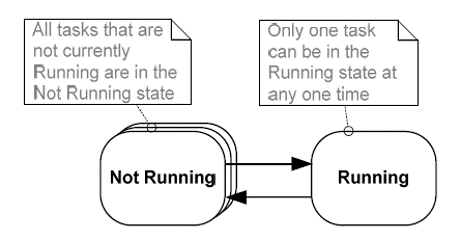
\includegraphics{figures/Fig_6_1_02rtos.png}
\bi
\ite Running state: the processor is
\ite executing its code.
\ite Not Running state: the task is dormant  its status having been saved ready for resuming execution the next time
\ei

\os{\newpage}



\item[{\rot\bf Creating Tasks}]~\\[-3ex]
\bi
\ite xTaskCreate() API function
\bi
\ite the most fundamental component in a multitasking system
\bi
\ite Probably the most complex of all API functions
\ite
\ei
\begin{lstlisting}[language=C]
 portBASE\_TYPE  xTaskCreate(
 pdTASK\_CODE 	pvTaskCode
 const signed char 	* const pcName
 unsigned short 		usStackDepth
 void 			*pvParameters
 unsigned portBASE\_TYPE uxPriority
 xTaskHandle 		*pxCreatedTask
 );
\end{lstlisting}
\ei
\ei

\os{\newpage}



\item[{\rot\bf All parameters}]~\\[-3ex]
\bi
\ite pvTaskCode
\bi
\ite a pointer to the function (just the function name) that implements the task.
\ei
\ite pcName
\bi
\ite A descriptive name for the task. It is not used by FreeRTOS but a debugging aid.
\ite configMAX\_TASK\_NAME\_LEN: the application defined constant that defines the maximum length a task name can task including the NULL terminator.
\ei
\ei

\os{\newpage}



\item[{\rot\bf All parameters}]~\\[-3ex]
\bi
\ite usStackDepth
\bi
\ite Each task has its own unique stack that is allocated by the kernel to the task when the task is created.
\ite The value specifies the number of words the task stack can hold.
\bi
\ite E.g. Cortex-M3 stack is 32 bits wide if usStackDepth is passed in as 100 400 bytes of stack space will be allocated (100*4 bytes)
\ei
\ite Size of the stack used by the idle task is defined by configMINIMAL\_STACK\_SIZE.
\bi
\ite Adjustable w.r.t. applications
\ei
\ei
\ei

\os{\newpage}



\item[{\rot\bf All parameters}]~\\[-3ex]
\bi
\ite pvParameters
\bi
\ite The value assigned to pvParameters will be the values passed into the task.
\ei
\ite uxPriority
\bi
\ite defines the priority at which the task will execute.
\ite Priorities can be assigned from 0 which is the lowest priority to (configMAX\_PRIOIRTIES-1) which is the highest priority.
\ite Passing a value above (configMAX\_PRIOIRTIES -1) will result in the priority being capped the maximum legitimate value.
\ei
\ei

\os{\newpage}



\item[{\rot\bf All parameters}]~\\[-3ex]
\bi
\ite pxCreatedTask
\bi
\ite pass out a handle to the created task then be used to refer the created task in API calls.
\bi
\ite E.g. change the task priority or delete the task
\ei
\ite Be set to NULL if no use for the task handle
\ite
\ei
\ite Two possible return values
\bi
\ite pdTRUE : task has been created successfully.
\ite errCOULD\_NOT\_ALLOCATE\_REQUIRED\_MEMORY
\bi
\ite Task has not been created as there is insufficient heap memory available for FreeRTOS to allocate enough RAM to hold the task data structures and stack.
\ei
\ei
\ei

\os{\newpage}



\item[{\rot\bf Example: Creating tasks}]~\\[-3ex]
\bi
\ite To demonstrate the steps of creating two tasks then starting the tasks executing.
\bi
\ite Tasks simply print out a string periodically using a crude null loop to create the periodic delay.
\ite Both tasks are created at the same priority and are identical except for the string they print out.
\ei
\ei

\os{\newpage}



\item[{\rot\bf Execution pattern of two Example 1 tasks}]~\\[-3ex]
\bi
\ite Both tasks are rapidly entering and exiting the Running state.
\ite Only one task can exist in the Running state at any one time.
\ei
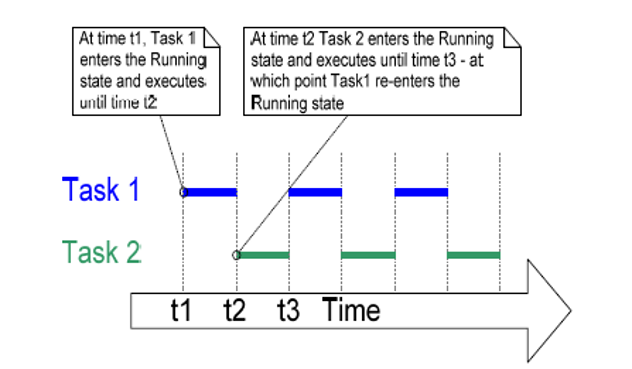
\includegraphics{figures/Fig_6_1_03rtos.png}

\os{\newpage}



\item[{\rot\bf Example 2 Using the task parameter}]~\\[-3ex]
\bi
\ite The two tasks in Example 1 are almost identical the only difference between them being the text string they print out.
\bi
\ite Remove such duplication by creating two instances of a single task implementation vTaskFunction.
\bi
\ite Each created instance will execute independently under the control of the FreeRTOS scheduler.
\ei
\ite The task parameter can then be used to pass into each task the string that it should print out.
\ei
\ei

\os{\newpage}



\item[{\rot\bf Example 2 Using the task parameter}]~\\[-3ex]
\bi
\ite First define a char string pcTextForTask1
\ite static const char *pcTextForTask1 = Task 1 is running.;
\ite Then in main(void) function change
\ite xTaskCreate( vTask1 Task 1 240 NULL 1 NULL );
\ite to
\ite xTaskCreate( vTaskFunction Task 1 240 (void*)pcTextForTask1 1 NULL );
\ite Create a task function vTaskFunction(void * pvParameters)
\ite char *pcTaskName;
\ite pcTaskName = (char *) pvParameters;
\ite
\ite
\ei

\os{\newpage}



\item[{\rot\bf Task priorities}]~\\[-3ex]
\bi
\ite uxPriority parameter of xTaskCreate() assigns an initial priority to the task being created.
\bi
\ite It can be changed after the scheduler has been started by using vTaskPrioritySet() API function
\ite
\ei
\ite configMax\_PRIORITIES in FreeRTOSConfig.h
\bi
\ite Maximum number of priorities
\ite Higher this value more RAM consumed
\ite Range: [0(low) configMAX\_PRIORITIES-1(high)]
\ite Any number of tasks can share the same priority
\ei
\ei

\os{\newpage}



\item[{\rot\bf Task priorities}]~\\[-3ex]
\bi
\ite To select the next task to run the scheduler itself must execute at the end of each time slice.
\bi
\ite Use a periodic interrupt called the tick (interrupt).
\ite Effectively set the length of time slice by the tick interrupt frequency -- configTICK\_RATE\_HZ in FreeRTOSConfig.h
\ei
\ite configTICK\_RATE\_HZ
\bi
\ite If it is 100(Hz) the time slice will be 10 ms.
\ite API always calls specify time in tick interrupts (ticks)
\ei
\ite portTICK\_RATE\_MS
\bi
\ite Convert time delays from milliseconds into the number of tick interrupts.
\ei
\ei

\os{\newpage}



\item[{\rot\bf Task priorities}]~\\[-3ex]
\bi
\ite When kernel itself is running the arrows in the above figure show the sequence of execution from task interrupt then from interrupt back to a next task.
\ei
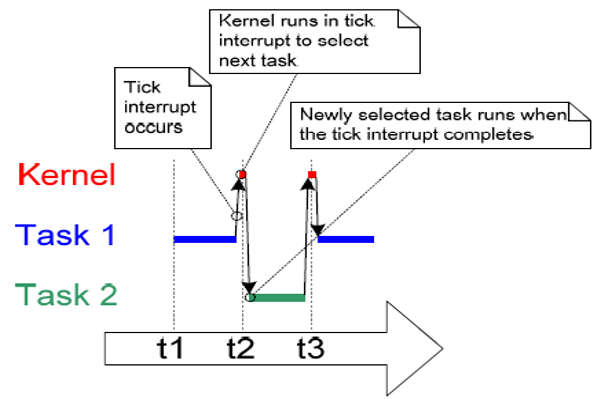
\includegraphics{figures/Fig_6_1_04rtos.png}

\os{\newpage}



\item[{\rot\bf Example 3. Experimenting with priorities}]~\\[-3ex]
\bi
\ite Scheduler always ensures that the highest priority task is able to run is the task selected to enter the Running state.
\bi
\ite In Example 1 and 2 two tasks have been created at the same priority so both entered and exited the Running state in turn.
\ite In this example the second task is set at priority 2.
\ei
\ei

\os{\newpage}



\item[{\rot\bf Example 3. Experimenting with priorities}]~\\[-3ex]
\bi
\ite In main() function change
\bi
\ite xTaskCreate( vTaskFunction Task 2 240 (void*)pcTextForTask2 1 NULL );
\ite To
\ite xTaskCreate( vTaskFunction Task 2 240 (void*)pcTextForTask2 2 NULL );
\ite
\ei
\ei

\os{\newpage}



\item[{\rot\bf Example 3. Experimenting with priorities}]~\\[-3ex]
\bi
\ite The scheduler always selects the highest priority task that is able to run.
\bi
\ite Task 2 has a higher priority than Task 1; so Task 2 is the only task to ever enter the Running state.
\ite Task 1 is to be "starved" of processing time of Task 2.
\ei
\ei
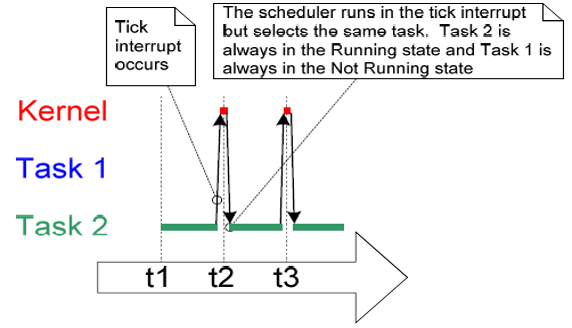
\includegraphics{figures/Fig_6_1_05rtos.png}

\os{\newpage}



\item[{\rot\bf"Continuous processing" task}]~\\[-3ex]
\bi
\ite So far the created tasks always have work to perform and have never had to wait for anything
\bi
\ite Always able to enter the Running state.
\ei
\ite This type of task has limited usefulness as they can only be created at the very lowest priority.
\bi
\ite If they run at any other priority they will tasks of lower priority  ever running at all.
\ei
\ite Solution: Event-driven tasks
\ei

\os{\newpage}



\item[{\rot\bf Expanding the "Not Running" state}]~\\[-3ex]
\bi
\ite An event-driven task
\bi
\ite has work to perform only after the occurrence of the event that triggers it
\ite Is not able enter the Running state before that event has occurred.
\ei
\ite The scheduler selects the highest priority task that is able to run.
\bi
\ite High priority tasks not being able to run means that the scheduler cannot select them and
\ite Must select a lower priority task that is able to run.
\ei
\ite Using event-driven tasks means that
\bi
\ite tasks can be created at different priorities without the highest priority tasks starving all the lower priority tasks.
\ei
\ei

\os{\newpage}



\item[{\rot\bf Full task state machine}]~\\[-3ex]

\begin{centering}
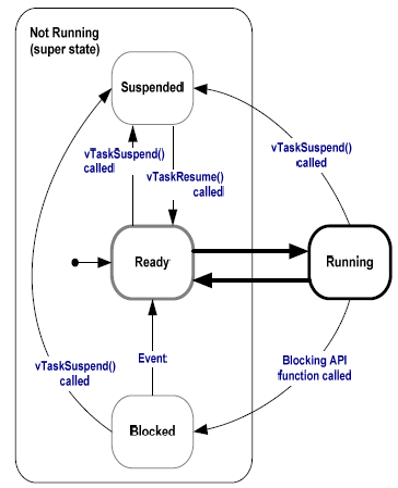
\includegraphics[height=12cm]{figures/Fig_6_1_08rtos.png}
\end{centering}
\os{\newpage}



\item[{\rot\bf Blocked state }]~\\[-3ex]
\bi
\ite Tasks enter this state to wait for two types of events
\bi
\ite Temporal (time-related) events: the event being either a delay expiring or an absolute time being reached.
\bi
\ite A task enter the Blocked state to wait for 10ms to pass
\ei
\ite Synchronization events: where the events originate from another task or interrupt
\bi
\ite A task enter the Blocked state to wait for data to arrive on a queue.
\ei
\ite Can block on a synchronization event with a timeout effectively block on both types of event simultaneously.
\bi
\ite A task waits for a maximum of 10ms for data to arrive on a queue. It leaves the Blocked state if either data arrives within 10ms or 10ms pass with no data arriving.
\ei
\ei
\ei

\os{\newpage}



\item[{\rot\bf Suspended state}]~\\[-3ex]
\bi
\ite Tasks in this state are not available to the scheduler.
\bi
\ite The only way into this state is through a call to the vTaskSuspend() API function
\ite The only way out this state is through a call to the vTaskResume() or vTaskResumeFromISR() API functions
\ei
\ei

\os{\newpage}



\item[{\rot\bf Ready state}]~\\[-3ex]
\bi
\ite Tasks that are in the "Not Running" state but are not Blocked or Suspended are said to be in the Ready state.
\bi
\ite They are able to run and therefore "ready" to run but are not currently in the Running state.
\ei
\ei

\os{\newpage}



\item[{\rot\bf Example 4 Using the Block state to create a delay}]~\\[-3ex]
\bi
\ite All tasks in the previous examples have been periodic
\bi
\ite They have delayed for a period and printed out their string before delay once more and so on.
\ite Delayed generated using a null loop
\bi
\ite the task effectively polled an incrementing loop counter until it reached a fixed value.
\ei
\ei
\ei

\os{\newpage}



\item[{\rot\bf Example 4 Using the Block state to create a delay}]~\\[-3ex]
\bi
\ite Disadvantages to any form of polling
\bi
\ite While executing the null loop the task remains in the Ready state"starving" the other task of any processing time.
\ite During polling the task does not really have any work to do but it still uses maximum processing time and so wastes processor cycles.
\ei
\ite This example corrects this behavior by
\bi
\ite replacing the polling null loop with a call to vTaskDelay() API function.
\ite setting INCLUDE\_vTaskDelay to 1 in FreeRTOSConfig.h
\ei
\ei

\os{\newpage}



\item[{\rot\bf vTaskDelay() API function}]~\\[-3ex]
\bi
\ite Place the calling task into the Blocked state for a fixed number of tick interrupts.
\bi
\ite The Blocked state task does not use any processing time so processing time is consumed only when there is work to be done.
\ite void vTaskDelay(portTickType xTicksToDelay);
\ite
\ei
\ite xTicksToDelay: the number of ticks that the calling task should remain in the Blocked state before being transitioned back into the Ready state.
\ite E.g if a task called vTaskDelay(100) while the tick count was 10000 it enters the Blocked state immediately and remains there until the tick count is 10100.
\ei

\os{\newpage}



\item[{\rot\bf vTaskDelay() API function}]~\\[-3ex]
\bi
\ite In void vTaskFunction(void *pvParameters)
\bi
\ite Change a NULL loop
\ite for( ul = 0; ul < mainDELAY\_LOOP\_COUNT; ul++ ) { }
\ite To
\ite vTaskDelay(250 / portTICK\_RATE\_MS);
\ite // a period of 250ms is being specified.
\ite Although two tasks are being created at different priorities both will now run.
\ei
\ei

\os{\newpage}



\item[{\rot\bf vTaskDelay() API function}]~\\[-3ex]
\bi
\ite Each time the tasks leave the Blocked state they execute for a fraction of a tick period before re-entering the Blocked state.
\bi
\ite Most of the time no application tasks are able to run and so no tasks can be selected to enter the Running state.
\ite The idle task will run to ensure there is always at least one task that is able to run.
\ei
\ei
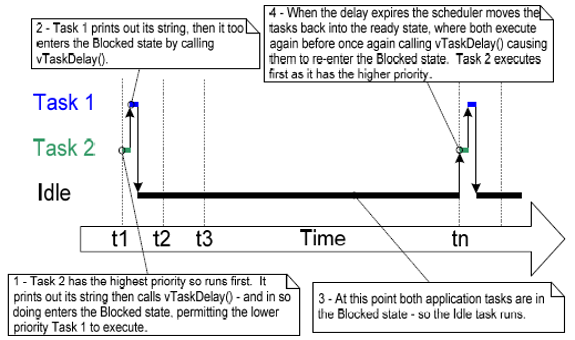
\includegraphics{figures/Fig_6_1_06rtos.png}

\os{\newpage}



\item[{\rot\bf Bold lines indicate the state transitions performed by the tasks in Example 4}]~\\[-3ex]

    \begin{centering}
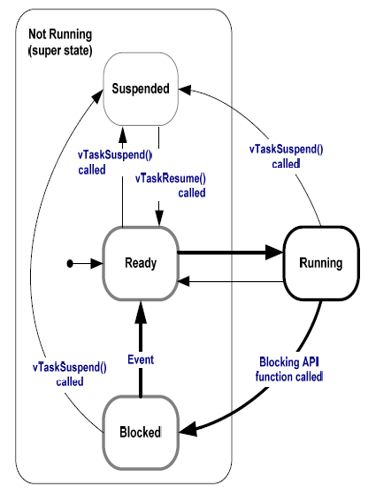
\includegraphics[height=6cm]{figures/Fig_6_1_07rtos.png}
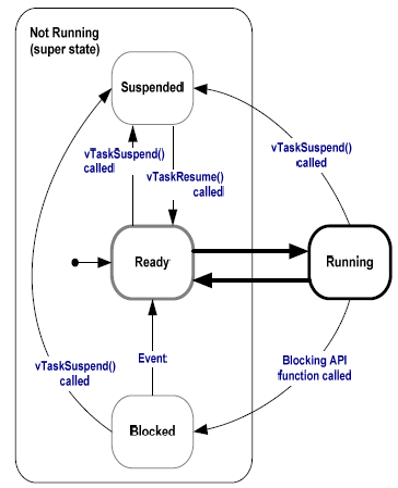
\includegraphics[height=6cm]{figures/Fig_6_1_08rtos.png}
\end{centering}

\bi
\ite Tasks 1+2
\ite Idle Task
\ei

\os{\newpage}



\item[{\rot \bf vTaskDelayUntil() API Function}]~\\[-3ex]

\bi
\ite Parameters to vTaskDelayUntil()
\bi
\ite specify the exact tick count value at which the calling task should be moved from the Blocked state into the Ready state.
\ite Be used when a fixed execution period is required.
\bi
\ite The time at which the calling task is unblocked is absolute rather than relative to when the function was called (as vTaskDelay())
\ei
\ite 	void vTaskDelayUntil(
\ite 		portTickType *pxPreviousWakeTime
\ite 		portTickType xTimeIncrement);
\ei
\ei
\os{\newpage}



\item[{\rot \bf vTaskDelayUntil() prototype}]~\\[-3ex]

\bi
\ite pxPreviousWakeTime
\bi
\ite Assume that vTaskDelayUtil() is being used to implement a task that executes periodically and with a fixed frequency.
\ite Holds the time at which the task left the Blocked state.
\ite Be used as a reference point to compute the time at which the task next leaves the Blocked state.
\ite The variable pointed by pxPreviousWakeTime is updated automatically not be modified by application code other than when the variable is first initialized.
\ei
\ei

\os{\newpage}



\item[{\rot \bf vTaskDelayUntil() prototype}]~\\[-3ex]
\bi
\ite xTimeIncrement
\bi
\ite Assume that vTaskDelayUtil() is being used to implement a task that executes periodically and with a fixed frequency - set by xTimeIncrement.
\ite Be specified in "ticks" . The constant portTICK\_RATE\_MS can be used to convert ms to ticks.
\ei
\ei

\os{\newpage}



\item[{\rot \bf Example 5 Converting the example tasks to use vTaskDelayUntil()}]~\\[-3ex]

\bi
\ite Two tasks created in Example 4 are periodic tasks.
\ite vTaskDelay() does not ensure that the frequency at which they run is fixed
\bi
\ite as the time at which the tasks leave the Blocked state is relative to when they call vTaskDelay().
\ei
\ei

\os{\newpage}



\item[{\rot\bf Example 5 Converting the example tasks to use vTaskDelayUntil()}]~\\[-3ex]
\bi
\ite In void vTaskFunction(void *pvParameters)
\bi
\ite Change
\ite vTaskDelay(250 / portTICK\_RATE\_MS);
\ite // a period of 250ms is being specified.
\ite To
\ite vTaskDelayUntil( \&xLastWakeTime (vTaskDelay(250 / portTICK\_RATE\_MS));
\ite /*xLastWakeTime is initialized with the current tick count before entering the infinite loop. This is the only time it is written to explicitly. */
\ite xLastWakeTime = xTaskGetTickCount();
\ite /*It is then updated within vTaskDelayUntil(); automatically */
\ei
\ei

\os{\newpage}



\item[{\rot\bf Example 6 Combining blocking and non-blocking tasks}]~\\[-3ex]
\bi
\ite Two tasks are created at priority 1.
\bi
\ite Always be either the Ready or the Running state as never making any API function calls.
\ite Tasks of this nature are called continuous processing tasks they always have work to do.
\ei
\ite A Third task is created at priority 2.
\bi
\ite Periodically prints out a string by using vTaskDelayUntil() to place itself into the Blocked state (blocking time 5) between each print iteration.
\ite
\ei
\ei

\os{\newpage}



\item[{\rot\bf Combining blocking and non-blocking tasks}]~\\[-3ex]

\bi
\ite void vContinuousProcessingTask(void * pvParameters) {
\ite   char *pcTaskName;
\ite   pcTaskName = (char *) pvParameters;
\ite   for (;;){ vPrintString(pcTaskName);
\ite         for( ul = 0; ul < 0xfff; ul++ ) { }
\ite   }}
\ite void vPeriodicTask(void * pvParameters) {
\ite   portTickType xLastWakeTime;
\ite   xLastWakeTime = xTaskGetTickCount();
\ite   for (;;){ vPrintString(Periodic task is running);
\ite      vTaskDelayUntil(\&xLastWakeTime
\ite                               (10/portTICK\_RATE\_MS));
\ite   }}
\ei

\os{\newpage}



\item[{\rot\bf Scheduling operations}]~\\[-3ex]

\vspace{2cm}
\begin{centering}
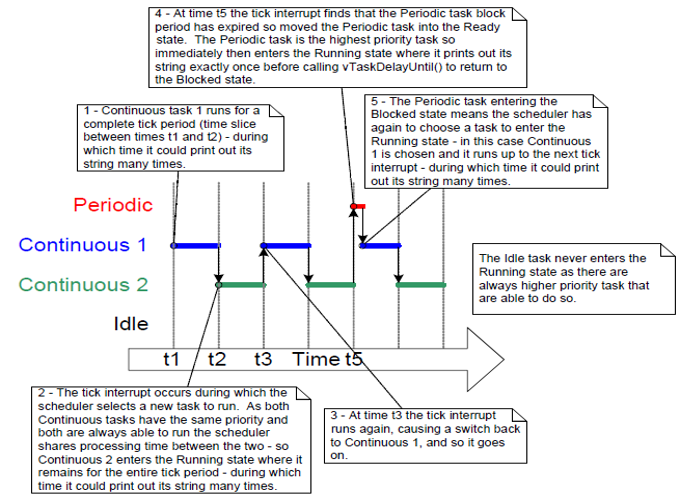
\includegraphics[width = 15 cm]{figures/Fig_6_1_09rtos.png}
\end{centering}
\os{\newpage}



\item[{\rot\bf Idle Task and the Idle task hook}]~\\[-3ex]

\bi
\ite An idle task is automatically created by the scheduler when vTaskStartScheduler() is called.
\bi
\ite Does very little more than site in a loop
\ite Has the lowest possible priority (zero) to ensure it never prevents a higher priority application task from entering the Running state
\ite Be transitioned out of the Running state as soon as a higher priority task enters the Ready state
\ei
\ei

\os{\newpage}



\item[{\rot\bf Idle Task}]~\\[-3ex]

\bi
\ite The Idle task is immediately swapped out to allow Task 2 to execute at the instant Task 2 leaves the Blocked state.
\bi
\ite Task 2 pre-empts the idle task automatically.
\ei
\ei
\begin{centering}
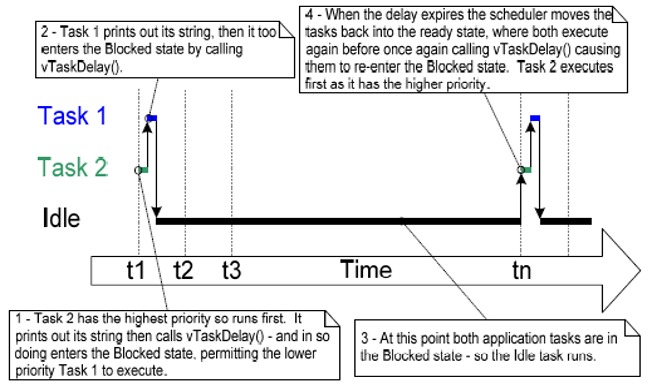
\includegraphics{figures/Fig_6_1_10rtos.png}
\end{centering}
\os{\newpage}



\item[{\rot\bf Idle Task Hook Functions}]~\\[-3ex]

\bi
\ite Add application specific functionality directly into the idle task by the use of an idle hook
\bi
\ite A function called automatically by the idle task once per iteration of the idle task loop
\ei
\ite Common uses for the Idle task hook
\bi
\ite Executing low priority background or continuous processing
\ite Measuring the amount of spare processing capacity
\ite Placing the processor into a low power mode providing an automatic method of saving power whenever no application processing to be performed.
\ei
\ei

\os{\newpage}



\item[{\rot\bf Limitations on the implementation of Idle Task Hook Functions}]~\\[-3ex]

\bi
\ite Rules idle task hook functions must adhere to
\bi
\ite Must never attempt to block or suspend.
\ite If the application uses vTaskDelete() the Idle task hook must always return to its caller within a reasonable time period.
\bi
\ite Idle task is responsible for cleaning up kernel resources after a task has been deleted.
\ite If the idle task remains permanently in the Idle hook function this clean-up cannot occur.
\ei
\ite Idle task hook functions have the name and prototype as
\bi
\ite void vApplicationIdleHook(void);
\ei
\ei
\ei

\os{\newpage}



\item[{\rot\bf Example 7 Defining an idle task hook function}]~\\[-3ex]

\bi
\ite Set configUSE\_IDLE\_HOOK to 1
\ite Add following function
\ite unsigned long ulIdleCycleCount = 0UL;
\ite /* must be called this name take no parameters and return void. */
\ite void vApplicationIdleHook (void) {
\ite    ulIdleCycleCount++;
\ite }
\ite In vTaskFunction() change
\ite 	vPrintString(pcTaskName) To
\ite      vPrintStringAndNumber(pcTaskName ulIdleCycleCount);
\ei

\os{\newpage}



\item[{\rot\bf Idle task and Idle Task Hook}]~\\[-3ex]

\bi
\ite Has the lowest priority possible to add functionality into the idle task vi idle hook
\bi
\ite Execute continuous processing
\ite Measuring spare processing capacity
\ite Placing the processor into a low power mode
\ei
\ite Two rules
\bi
\ite Never block or suspend; must return to its caller within a reasonable time period as it needs to clean up kernel resources after a deleted task.
\ei
\ei

\os{\newpage}



\item[{\rot\bf Change the priority of a task}]~\\[-3ex]

\bi
\ite vTaskPrioritySet(xTaskHandle pxTask unsigned portBASE\_TYPE uxNewPriority);
\ite Be used to change the priority of any task after the scheduler has been started.
\ite Available if INCLUDE\_vTaskPrioritySet  is set 1.
\ei
\ite Two parameters
\bi
\ite pxTask: Handle of the task whose priority is being modified. A task can change its own priority by passing NULL in place of a valid task handle.
\ite uxNewPriority:  the priority to be set.
\ei


\os{\newpage}



\item[{\rot\bf Change the priority of a task}]~\\[-3ex]

\bi
\ite unsigned portBASE\_TYPE uxTaskPriorityGet(xTaskHandle pxTask);
\bi
\ite Be used to query the priority of a task
\ite Available if INCLUDE\_vTaskPriorityGet is set 1
\ite pxTask: Handle of the task whose priority is being modified. A task can query its own priority by passing NULL in place of a valid task handle.
\ite Returned value: the priority currently assigned to the task being queried
\ei
\ei

\os{\newpage}



\item[{\rot\bf Example: Changing task priorities}]~\\[-3ex]

\bi
\ite Demonstrate the scheduler always selects the highest Ready state task to run
\bi
\ite by using the vTaskPrioritySet() API function to change the priority of two tasks relative to each other.
\ei
\ite Two tasks are created at two different priorities.
\bi
\ite Neither task makes any API function calls that cause it to enter the Blocked state
\bi
\ite So both are in either Ready or Running state.
\ite So the task with highest priority will always be the task selected by the scheduler to be in Running state
\ei
\ei
\ei

\os{\newpage}



\item[{\rot\bf Expected Behavior of Example 8}]~\\[-3ex]

\bi
\ite Task 1 is created with the highest priority to be guaranteed to run first. Task 1 prints out a couple of strings before raising the priority of Task 2 to above its own priority.
\ite Task2 starts to run as it has the highest relative priority.
\ite Task 2 prints out a message before setting its own priority back to below that of Task 1.
\ite Task 1 is once again the highest priority task so it starts to run and forcing Task 2 back into the Ready state.
\ei

\os{\newpage}



\item[{\rot\bf Example 8 Continued}]~\\[-3ex]

\bi
\ite Declare a global variable to hold the handle of Task 2.
\bi
\ite xTaskHandle xTask2Handle;
\ei
\ite In main() function create two tasks
\bi
\ite xTaskCreate(vTask1 Task 1 240
\ite 			NULL 2 NULL);
\ite xTaskCreate(vTask2 Task 2 240
\ite 			NULL 1 \&xTask2Handle);
\ei
\ite
\ei

\os{\newpage}



\item[{\rot\bf Initialization}]~\\[-3ex]

\bi
\ite Change vTask1 by initialization
\bi
\ite unsigned portBASE\_TYPE uxPriority;
\ite uxPriority = uxTaskPriorityGet(NULL);
\ei
\ite And adding to the infinite loop
\bi
\ite vTaskPrioritySet(xTaskHandl1 (uxPriority+1));
\ei
\ite Change vTask2 by initialization
\bi
\ite unsigned portBASE\_TYPE uxPriority;
\ite uxPriority = uxTaskPriorityGet(NULL);
\ei
\ite And adding to the infinite loop
\bi
\ite vTaskPrioritySet(NULL (uxPriority-2));
\ei
\ei

\os{\newpage}



\item[{\rot\bf Task with changing priority: execution sequence}]~\\[-3ex]

\vspace{2cm}
\begin{centering}
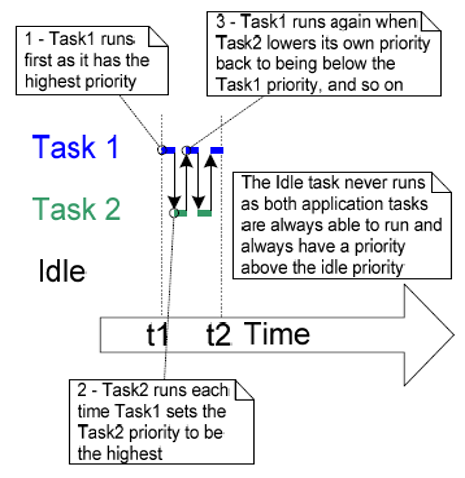
\includegraphics[height=9 cm]{figures/Fig_6_1_11rtos.png}
\end{centering}

\os{\newpage}



\item[{\rot\bf Deleting a task}]~\\[-3ex]

\bi
\ite Deleted tasks no longer exist and cannot enter the Running state again.
\ite Idle task is responsible to automatically free memory allocated by kernel to tasks that have been deleted.
\bi
\ite Remember if applications use vTaskDelete() do not completely starve the idle task of all processing time.
\ei
\ite Note: any memory or other resource that the application task allocates itself must by be freed explicitly by the application code.
\ei

\os{\newpage}



\item[{\rot\bf vTaskDelete() API function}]~\\[-3ex]

\bi
\ite Function prototype
\bi
\ite void vTaskDelete(xTaskHandle  pxTaskToDelete);
\ite pxTaskToDelete: Handle of the task that is to be deleted. A task can delete itself by passing NULL in place of valid task handle.
\ei
\ite Available only when INCLUDE\_vTaskDelete set 1
\ei

\os{\newpage}



\item[{\rot\bf Example: Deleting tasks (Behavior)}]~\\[-3ex]

\bi
\ite Task 1 is created by main() with priority 1. When it runs it creates Task 2 at priority 2. Task 2 as the highest priority task starts to execute immediately.
\ite Task 2 does nothing but delete itself by passing NULL or its own task handle.
\ite When Task 2 has been deleted Task 1 is again the highest priority task so continues executing - at which point it calls vTaskDelay() to block for a short period.
\ite The idle task executes while Task 1 is in the blocked state and frees the memory that was allocated to the now deleted Task 2.
\ite When Task 1 leaves the blocked state it again becomes the highest priority Ready state task and preempts the Idle task. Then start from Step1 again.
\ei

\os{\newpage}



\item[{\rot\bf Execution sequence}]~\\[-3ex]

\vspace{2cm}
\begin{centering}
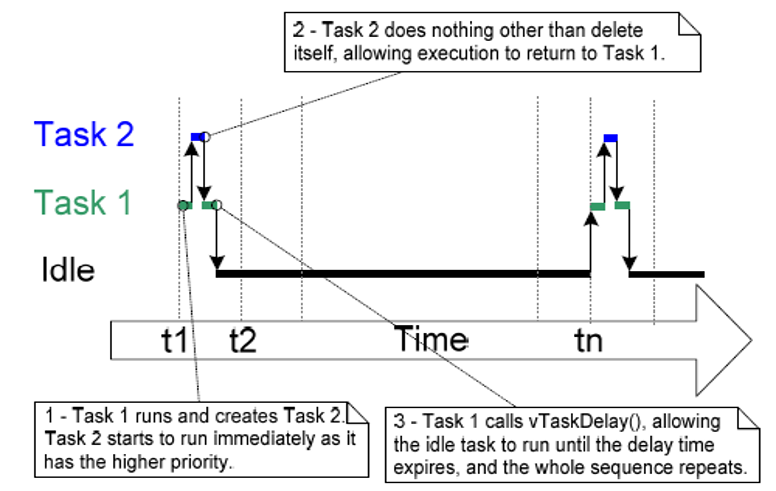
\includegraphics[height = 9 cm]{figures/Fig_6_1_12rtos.png}
\end{centering}
\os{\newpage}



\item[{\rot\bf Memory Management}]~\\[-3ex]

\bi
\ite Does not permit memory to be freed once it has been allocated.
\ite Subdivide a single array into smaller blocks. Total size of the array (heap) is set by configTOTAL\_HEAP\_SIZE
\ite xPortGetFreeHeapSize() returns the total amount of heap space that remains unallocated.
\ei

\os{\newpage}



\item[{\rot\bf Heap\_2.c}]~\\[-3ex]

\bi
\ite Allow previously allocated blocks to be freed.
\ite Does not combine adjacent free blocks into a single large block.
\ei

\os{\newpage}



\item[{\rot\bf Summary - Prioritized pre-emptive scheduling}]~\\[-3ex]

\bi
\ite Examples illustrate how and when FreeRTOS selects which task should be in the Running state.
\bi
\ite Each task is assigned a priority.
\ite Each task can exist in one of several states.
\ite Only one task can exist in the Running state at any one time.
\ite The scheduler always selects the highest priority Ready state task to enter the Running state.
\ei
\ei

\os{\newpage}



\item[{\rot\bf Fixed priority Pre-emptive scheduling}]~\\[-3ex]

\bi
\ite Fixed priority
\bi
\ite Each task is assigned a priority that is not altered by the kernel itself (only tasks can change priorities)
\ei
\ite Pre-emptive
\bi
\ite A task entering the Ready state or having its priority altered will always pre-empt the Running state task if the Running state task has a lower priority.
\ei
\ei

\os{\newpage}



\item[{\rot\bf Tasks in the Blocked state}]~\\[-3ex]

\bi
\ite Tasks can wait in the Blocked state for an event and are automatically moved back to the Ready state when the event occurs.
\ite Temporal events
\bi
\ite Occur at a particular time e.g. a block time expires.
\ite Generally be used to implement periodic or timeout behavior.
\ei
\ite Synchronization events
\bi
\ite Occur when a task or ISR sends info to a queue or to one of the many types of semaphore.
\ite Generally be used to signal asynchronous activity such as data arriving at a peripheral.
\ei
\ite
\ei

\os{\newpage}



\item[{\rot\bf Semaphores \& Queues}]~\\[-3ex]

\bi
\ite Introduction to task synchronization
\ite Semaphores and mutexs of FreeRTOS
\ite Queues of FreeRTOS
\ei

\os{\newpage}



\item[{\rot\bf Why Synchronization?}]~\\[-3ex]

\bi
\ite Synchronization may be used to solve:
\bi
\ite Mutual exclusion
\ite Control flow
\ite Data flow
\ei
\ite Synchronization mechanisms include:
\bi
\ite Message queues
\ite Semaphores
\ite Mutexs
\ite Events
\ei
\ite Correct synchronization mechanism depends on the synchronization issue being addressed
\ei


\os{\newpage}



\item[{\rot\bf Mutual Exclusion}]~\\[-3ex]

\bi
\ite Problem: multiple tasks may simultaneously need to access the same resource
\bi
\ite Resource may be code data peripheral etc.
\ite Need to allow the shared resource exclusively accessible to only one task at a time
\ei
\ite How to do?
\bi
\ite Allowing only one task to lock the resource and the rest have to wait for the resource to be unlocked
\ite Common mechanisms: lock/unlock mutex semaphore
\ei
\ei

\os{\newpage}



\item[{\rot\bf Control Flow Synchronization}]~\\[-3ex]

\bi
\ite Problem: a task or ISR may need to resume the execution of one or more other tasks so that tasks execute in an application-controlled order
\bi
\ite Mutual exclusion is used to prevent another task from running while control flow is used to allow another task to run often specific tasks
\ei
\ite How to do?
\bi
\ite Common mechanisms: post/wait signal event
\ei
\ei

\begin{centering}
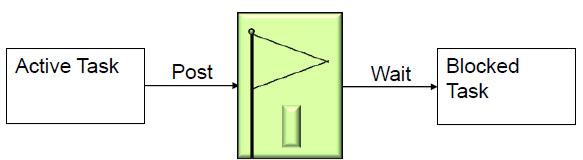
\includegraphics[height=4cm]{figures/Fig_6_1_13rtos.png}
\end{centering}

\os{\newpage}



\item[{\rot\bf Data Flow Synchronization}]~\\[-3ex]

\bi
\ite Problem: a task or ISR may need to pass some data to one or more other specific tasks so that data may be processed in an application-specified order
\ite How to do?
\bi
\ite May be accomplished indirectly through control flow synchronization
\ite Common mechanisms: queues signal post/wait
\ei
\ei

\os{\newpage}



\item[{\rot\bf Outline}]~\\[-3ex]

\bi
\ite Introduction to task synchronization
\ite Semaphores and mutexs of FreeRTOS
\bi
\ite Binary semaphores
\ite Counting semaphores
\ite Mutex
\ei
\ite Queues of FreeRTOS
\ei

\os{\newpage}



\item[{\rot\bf Semaphores}]~\\[-3ex]

\bi
\ite Semaphores are used to:
\bi
\ite Control access to a shared resource (mutual exclusion)
\ite Signal the occurrence of an event
\ite Allow two tasks to synchronize their activities
\ei
\ite Basic idea
\bi
\ite A semaphore contains a number of tokens. The code needs to acquire one in order to continue execution
\ite If all the tokens of the semaphore are used the requesting task is suspended until some tokens are released by their current owners
\ei
\ei

\includegraphics{figures/Fig_6_1_14rtos.png}

\os{\newpage}



\item[{\rot\bf How Semaphores Work?}]~\\[-3ex]

\bi
\ite A semaphore has:
\bi
\ite Counter: maximum number of concurrent accesses
\ite Queue: for tasks that wait for access
\ei
\ite If a task requests (waits for) a semaphore
\bi
\ite if counter > 0 then (1) the counter is decremented by 1 and (2) task gets the semaphore and proceed to do work
\ite Else task is blocked and put in the queue
\ei
\ite If a task releases (posts) a semaphore
\bi
\ite if there are tasks in the semaphore queue then appropriate task is readied according to queuing policy
\ite Else counter is incremented by 1
\ei
\ei

\os{\newpage}



\item[{\rot\bf Binary Semaphores}]~\\[-3ex]

\bi
\ite Semaphores with counter = 1 used for mutual exclusion and synchronization
\bi
\ite For synchronization purpose a binary semaphore can be think of as a queue that can only hold one item
\bi
\ite The queue can only be empty or full (hence binary)
\ite Tasks using the queue don't care what the queue holds only want to know if the queue is empty or full
\ite  If more than one task blocks on the same semaphore then the task with the highest priority will be the task that is unblocked the next time the semaphore becomes available
\ei
\ei
\ei

\os{\newpage}



\item[{\rot\bf Binary Semaphores and Interrupts}]~\\[-3ex]

\bi
\ite The best way to handle complex events triggered by interrupts is to not do the code in the ISR
\bi
\ite Create a task that is blocking on a binary semaphore
\ite When the interrupt happens the ISR just sets (gives) the semaphore and exits
\ite Task can now be scheduled like any other
\bi
\ite No need to worry about nesting interrupts and interrupt priority
\ei
\ite This is called Deferred Interrupt Processing
\ei
\ei
\os{\newpage}



\item[{\rot\bf Binary Semaphores and Interrupts}]~\\[-3ex]

\bi
\ite Figure from Using the FreeRTOS Real Time Kernel (a pdf book) fair use claimed.
\ei

\begin{centering}
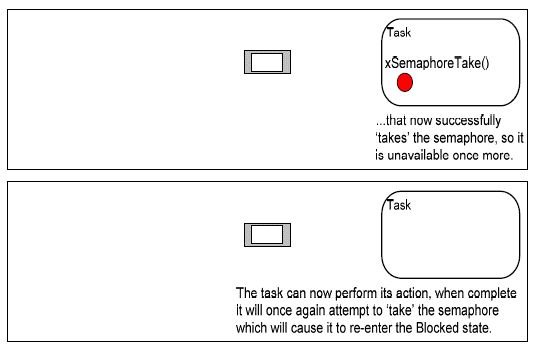
\includegraphics[width = 9 cm]{figures/Fig_6_1_15rtos.png}
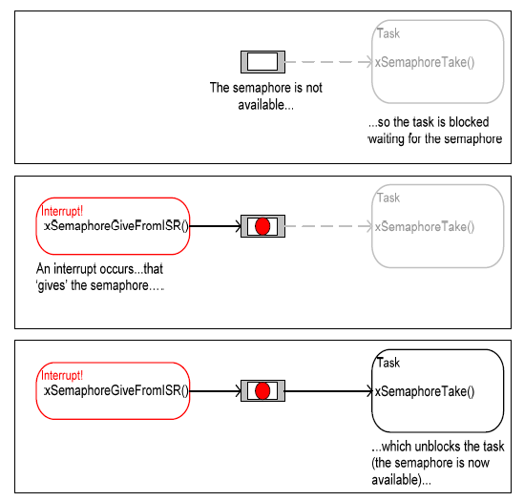
\includegraphics[width = 9 cm]{figures/Fig_6_1_16rtos.png}
\end{centering}

\os{\newpage}



\item[{\rot\bf Create a Binary Semaphore}]~\\[-3ex]

\bi
\ite SemaphoreHandle\_t xSemaphoreCreateBinary(void);
\ite Function to create a binary semaphore
\bi
\ite The semaphore is created in the 'empty' state
\ite A binary semaphore need not be given back once obtained so task synchronization can be implemented by one task/interrupt continuously 'giving' the semaphore while another continuously 'takes' the semaphore
\ite Binary semaphores are assigned to variables of type SemaphoreHandle\_t and can be used in any API function that takes a parameter of this type
\ei
\ei

\os{\newpage}



\item[{\rot\bf Set a Binary Semaphore}]~\\[-3ex]

\bi
\ite xSemaphoreGiveFromISR(
\ite   SemaphoreHandle\_t xSemaphore
\ite   signed BaseType\_t *pxHigherPriorityTaskWoken)
\ite Set (give) a semaphore
\bi
\ite Can be used from an ISR
\ite xSemaphore: handle to the semaphore being released
\ite pxHigherPriorityTaskWoken: set to pdTRUE if giving the semaphore caused a task of a higher priority to unblock causing a context switch
\ei
\ei

\os{\newpage}



\item[{\rot\bf Reset a Binary Semaphore}]~\\[-3ex]

\bi
\ite xSemaphoreTake(	xSemaphoreHandle xSemaphore
\ite        	portTickType xBlockTime)
\ite Reset (take) a semaphore
\bi
\ite xSemaphore: handle to the semaphore being taken
\ite xBlockTime: time in ticks to wait for the semaphore to become available
\bi
\ite A block time of zero can be used to poll the semaphore
\ei
\ei
\ei

\os{\newpage}



\item[{\rot\bf Example of Binary Semaphores}]~\\[-3ex]

\vspace{1cm}
\begin{tabular}{|l|} \hline
vSemaphoreHandle binary\_sem; //Global handler
void one\_sec\_isr(void){ // an ISR
  xSemaphoreGiveFromISR(binary\_sem NULL);		
}
void sem\_task(void *p){
  while(1)
    if(xSemaphoreTake(binary\_sem999999)) puts(Tick!);
}
int main(void){
    vSemaphoreCreateBinary(binary\_sem);
    xTaskCreate(sem\_task (signed char*)) t1 2048
         NULL 1 NULL);
    vTaskStartScheduler();
    return 0;	
}  \\ \hline
\end{tabular}


\os{\newpage}



\item[{\rot\bf Counting Semaphores}]~\\[-3ex]

\bi
\ite Typically used for two things:
\ite Counting events:
\bi
\ite An event handler will "give" a semaphore each time an event occurs and a handler task will 'take' a semaphore each time it processes an event
\ei
\ite Resource management:
\bi
\ite The count value indicates number of available resources
\ite To get a resource a task must obtain (take) a semaphore
\ite When a task finishes with the resource it 'gives' the semaphore back
\ei
\ite SemaphoreHandle\_t xSemaphoreCreateCounting( UBaseType\_t uxMaxCount    UBaseType\_t uxInitialCount)
\ei

\os{\newpage}



\item[{\rot\bf Priority Inversion}]~\\[-3ex]

\bi
\ite LPT starts running and acquires the semaphore.
\ite Now HPT is created and it preempts LPT and starts running. It makes the request to acquire the semaphore. Since the semaphore is already with LPT HPT goes to blocked state.
\ite LPT starts executing again and releases the semaphore.
\ite Immediately the HPT comes out of the blocked state and starts executing.
\ite It releases the semaphore and runs for some time and deletes itself.
\ite Now control goes back to LPT which completes its job and deletes itself.
\ite Finally the scheduler is left out with the idle task and it keeps running.
\ei

\os{\newpage}



\item[{\rot\bf Priority Inversion}]~\\[-3ex]

\vspace{1cm}
\begin{centering}
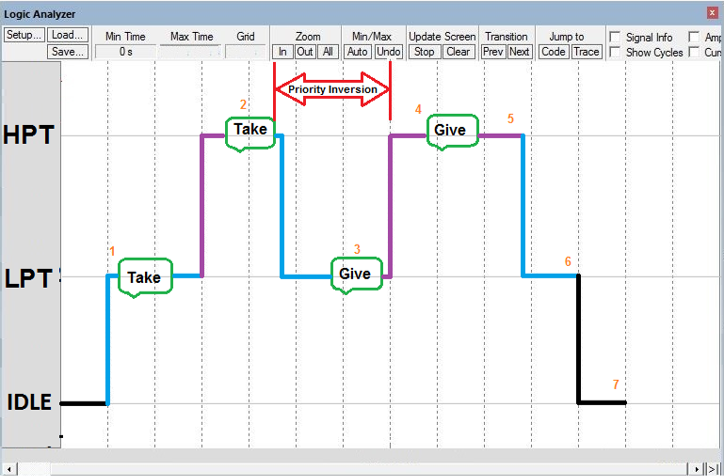
\includegraphics[width=16cm]{figures/Fig_6_1_prio1_rtos}
\end{centering}

\os{\newpage}



\item[{\rot\bf Extended Priority Inversion}]~\\[-3ex]

\bi
\ite LPT starts running and acquires the semaphore.
\ite Now HPT is created and it preempts LPT and starts running. It makes the request to acquire the semaphore. Since the semaphore is already with LPT HPT goes to blocked state.
\ite LPT starts executing again and waits for an event(packet to be received).
\ite Now the Idle task starts running. Now the HPT is starved because of LPT and Idle task.
\ite LPT comes out of blocked state as the event(wait time/packet is received) has occurred. Now it releases the semaphore.
\ite Immediately the HPT comes out of the blocked state and starts executing. It releases the semaphore and runs for some time and deletes itself.
\ite Now control goes back to LPT which completes its job and deletes itself.
\ite Finally the scheduler is left out with the idle task and it keeps running.
\ei

\os{\newpage}



\item[{\rot\bf Extended Priority Inversion}]~\\[-3ex]

\vspace{1cm}
\begin{centering}
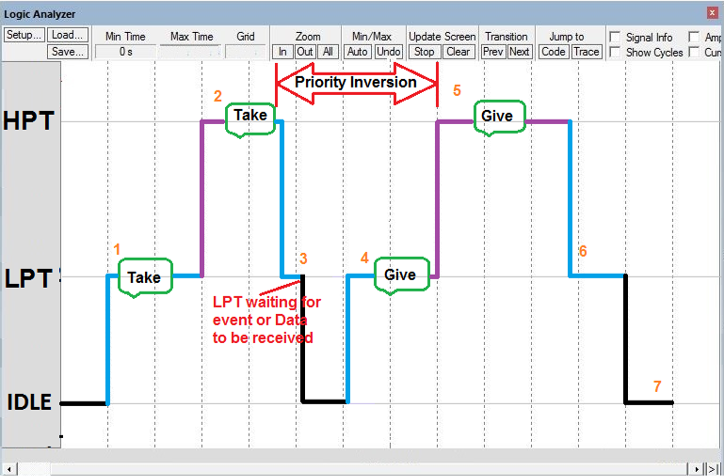
\includegraphics[width=16cm]{figures/Fig_6_1_prio2_rtos}
\end{centering}
\os{\newpage}



\item[{\rot\bf Worst Case Priority Inversion}]~\\[-3ex]
\bi
\ite LPT starts running and acquires the semaphore.
\ite Now HPT is created and it preempts LPT and starts running. It makes the request to acquire the semaphore. Since the semaphore is already with LPT HPT goes to blocked state.
\ite LPT starts executing again and creates an MPT tasks.
\ite MPT preempts the LPT and starts running. At this point the HPT is starved because of LPT and MPT. MPT completes its job and deletes itself.
\ite LPT comes out of blocked state and releases the semaphore.
\ite Immediately the HPT comes out of the blocked state and starts executing. It releases the semaphore and runs for some time and deletes itself.
\ite Now control goes back to LPT which completes its job and deletes itself.
\ite Finally the scheduler is left out with the idle task and it keeps running.
\ei

\os{\newpage}



\item[{\rot\bf Worst Case Priority Inversion}]~\\[-3ex]

\vspace{1cm}
\begin{centering}
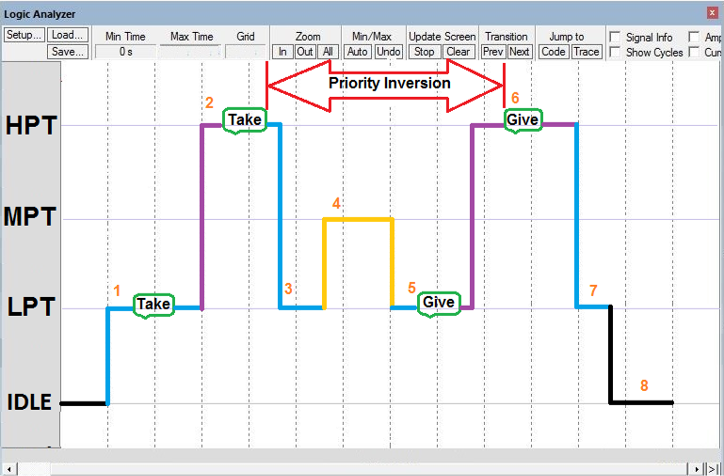
\includegraphics[width=16cm]{figures/Fig_6_1_prio3_rtos}
\end{centering}
\os{\newpage}



\item[{\rot\bf Priority Inheritance}]~\\[-3ex]
\bi
\ite As soon as the HPT makes a request to semaphore which is allocated to an LPT then the priority of LPT is temporarily increased to that of HPT. Once the LPT releases the semaphore its priority will be restored. Because of this the MPT is never allowed to interfere during the priority inversion(between LPT\&HPT). -> Mutex!
\ite LPT starts running and acquires the semaphore.
\ite Now HPT is created and it preempts LPT and starts running. It makes the request to acquire the semaphore. Since the semaphore is already with LPT HPT goes to blocked state and LPT's priority is temporarily raised to that of HPT.
\ite LPT starts executing again and creates an MPT tasks. It keeps running as its priority is currently higher than MPT. It releases the semaphore and its priority is restored back to lower value.
\ite Immediately the HPT comes out of the blocked state and starts executing.
\ite HPT releases the semaphore and runs for some time and deletes itself.
\ite Now scheduler is left with LPTMPT and IDLE task. MPT starts running and deletes itself after completing its job.
\ite Now control goes back to LPT which completes its job and deletes itself.
\ite Finally the scheduler is left out with the idle task and it keeps running.
\ei

\os{\newpage}



\item[{\rot\bf Priority Inheritance}]~\\[-3ex]

\vspace{1cm}
\begin{centering}
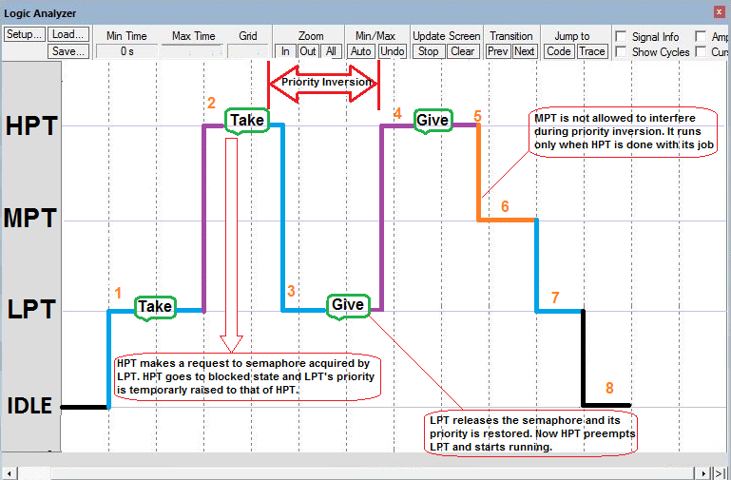
\includegraphics[width=16cm]{figures/Fig_6_1_prio4_rtos}
\end{centering}
\os{\newpage}



\item[{\rot\bf Mutex}]~\\[-3ex]
\bi
\ite Mutexes are used for mutual exclusion so that only one task at a time uses a shared resource e.g. file data device ...
\bi
\ite To access the shared resource a task locks the mutex associated with the resource
\ite The task owns the mutex until it unlocks the mutex
\ei
\ei
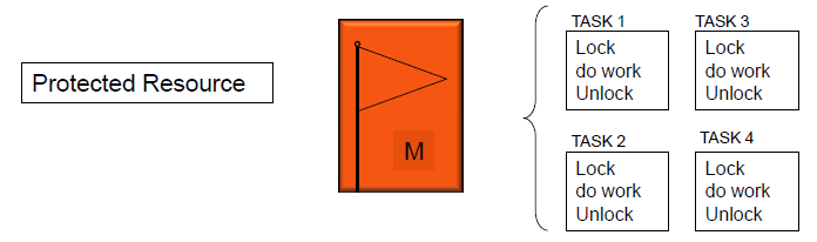
\includegraphics[width=16cm]{figures/Fig_6_1_17rtos.png}

\os{\newpage}



\item[{\rot\bf Mutex}]~\\[-3ex]
\bi
\ite Mutex acts like a token used to guard a resource
\bi
\ite When a task wishes to access the resource it must first obtain ('take') the token
\ite When the task has finished with the resource it must 'give' the token back - allowing other tasks the opportunity to access the same resource
\ei
\ite Mutexes are binary semaphores that include a priority inheritance mechanism
\bi
\ite If a high priority task blocks while attempting to obtain a mutex (token) that is currently held by a lower priority task then the priority of the task holding the token is temporarily raised to that of the blocking task
\ei
\ei

\os{\newpage}



\item[{\rot\bf Priority Inversion}]~\\[-3ex]
\bi
\ite Assume priority of T1 \> priority of T9
\bi
\ite If T9 has exclusive access T1 has to wait until T9 releases resource inverting priority can raise priority of T9
\ei
\ei
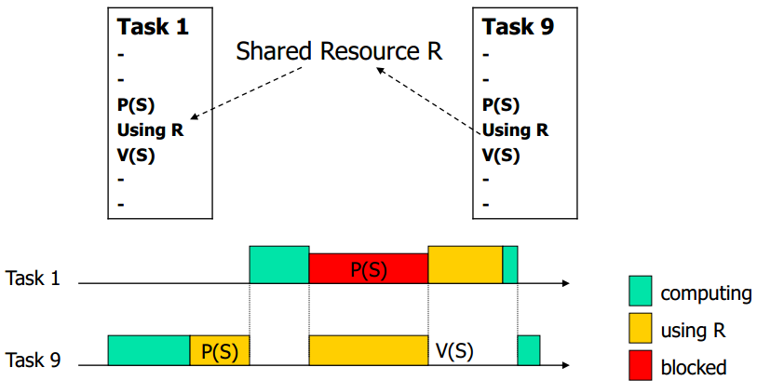
\includegraphics[width=14cm]{figures/Fig_6_1_18rtos.png}
\bi
\ite T1 has higher priority and preempts T9
\ei
\bi
\ite Critical section
\ei
\bi
\ite (critical section)
\ei

\os{\newpage}



\item[{\rot\bf Example of Mutex (1/3)}]~\\[-3ex]

\vspace{1cm}
\begin{tabular}{|l|} \hline
xSemaphoreHandle gatekeeper = 0; //Global handler\\

void task\_1(void *p)\{\\
  while(1)\{\\
    if(xSemaphoreTake(gatekeeper 1000))\{\\
      puts(Task 1 got access);\\
	access\_precious\_resource(); // critical section\\
	xSemaphoreGive(gatekeeper);  \}\\
    else\{\\
	puts(Task 1 failed to get access within 1000ms);\\
    \}\\
    vTaskDelay(1000);\\
      /*Without delay Task 1 will get key immediately\\
          after releasing the key */ \\
  \}\\
\}  \\ \hline
\end{tabular}


\os{\newpage}



\item[{\rot\bf Example of Mutex (2/3)}]~\\[-3ex]

\vspace{1cm}
\begin{tabular}{|l|} \hline
void task\_2(void *p)\{ \\
  while(1)\{\\
    if(xSemaphoreTake(gatekeeper 1000))\{ \\
      puts(Task 2 got access);\\
	access\_precious\_resource(); // critical section\\
	xSemaphoreGive(gatekeeper); \}\\
    else\{\\
	puts(Task 2 failed to get access within 1000ms);\\
    \}\\
    vTaskDelay(1000);\\
    /*Without delay task 2 will get key immediately\\
          after releasing the key */\\
   \}\\
\}  \\ \hline
\end{tabular}


\os{\newpage}



\item[{\rot\bf Example of Mutex (3/3)}]~\\[-3ex]

\vspace{1cm}
\begin{tabular}{|l|} \hline
int main(void)\{\\
  gatekeeper = xSemaphoreCreateMutex();\\
\\
  /*Create tasks with priority 1 for both users*/\\
  xTaskCreate(task\_1 (signed char*)) t1 1024\\
      NULL 1 NULL);\\
  xTaskCreate(task\_2 (signed char*)) t2 1024\\
      NULL 1 NULL);\\
	\\
  vTaskStartScheduler();\\
  return 0;\\
\}  \\ \hline
\end{tabular}


\os{\newpage}



\item[{\rot\bf Outline}]~\\[-3ex]
\bi
\ite Introduction to task synchronization
\ite Semaphores and mutexs of FreeRTOS
\ite Queues of FreeRTOS
\ei

\os{\newpage}



\item[{\rot\bf FreeRTOS Queues}]~\\[-3ex]

\bi
\ite Queues are the primary form of inter-task communications in FreeRTOS
\bi
\ite Can be used to send messages between tasks and between interrupts and tasks
\ite In most cases used as thread safe FIFO (First In First Out) buffers with new data being sent to the back of the queue although data can also be sent to the front.
\ei
\ei
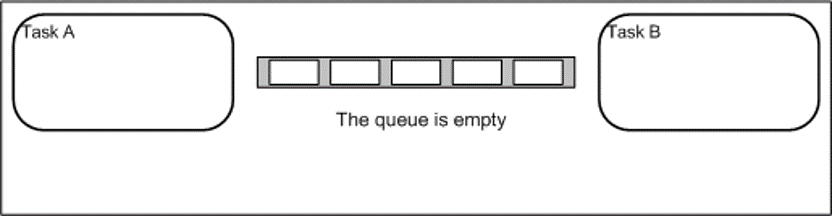
\includegraphics[width=16cm]{figures/Fig_6_1_19rtos.png}

\os{\newpage}



\item[{\rot\bf FreeRTOS Queues}]~\\[-3ex]

\bi
\ite Queues store a finite number of fixed-size data
\bi
\ite May be read and written by different tasks but do not belong to any task
\ite \# of items and item size determined at queue create time
\ite Sending/receiving items are by copy not reference
\ei
\ite Queue functions
\bi
\ite Create queues: xQueueCreate() vQueueDelete()
\ite Send/receive data to/from queues: xQueueSend() xQueueSendToBack() xQueueReceive() xQueueReceiveFromISR()
\ite Queue management/number of items in a queue
\ite Blocking on a queue/effect of priority
\ei
\ei

\os{\newpage}



\item[{\rot\bf Blocking on Queues}]~\\[-3ex]

\bi
\ite Queue APIs permit a block time to be specified
\ite When read from an empty queue
\bi
\ite Task will be placed into the Blocked state
\ite Until data is available on the queue or block time expires
\ei
\ite When write to a full queue
\bi
\ite Task will be placed into the Blocked state
\ite Until space is available in the queue or block time expires
\ei
\ite If more than one task block on the same queue then the task with the highest priority will be the task that is unblocked first
\ei

\os{\newpage}



\item[{\rot\bf Queue Creation}]~\\[-3ex]

\bi
\ite QueueHandle\_t xQueueCreate(
\ite     UBaseType\_t uxQueueLength
\ite     UBaseType\_t uxItemSize);
\ite Creates a new queue instance
\bi
\ite Allocates queue storage and returns a handle
\ite uxQueueLength: maximum number of items that the queue can contain
\ite uxItemSize: number of bytes that each item in the queue will require
\bi
\ite Items are queued by copy not by reference so this is the number of bytes that will be copied for each posted item
\ei
\ite Each item on the queue must be the same size
\ei
\ei

\os{\newpage}



\item[{\rot\bf Send Data through Queues}]~\\[-3ex]

\bi
\ite BaseType\_t xQueueSend(QueueHandle\_t xQueue
\ite       const void * pvItemToQueue
\ite       TickType\_t xTicksToWait);
\ite Post an item on a queue
\bi
\ite The item is queued by copy not by reference
\ite Must not be called from an interrupt service routine
\ite xQueue:  queue handle to which the item is to be posted
\ite pvItemToQueue: pointer to item to be placed on queue
\ite xTicksToWait: max. time (in ticks) that task should block waiting for space to become available should it is full
\ite If INCLUDE\_vTaskSuspend is set to "1" then specifying the block time as portMAX\_DELAY will block task indefinitely
\ei
\ei

\os{\newpage}



\item[{\rot\bf Receive Data through Queues}]~\\[-3ex]

\bi
\ite BaseType\_t xQueueReceive(
\ite     QueueHandle\_t xQueue void *pvBuffer
\ite     TickType\_t xTicksToWait);
\ite Receive an item from a queue
\bi
\ite The item is received by copy so a buffer of adequate size must be provided
\ite Must not be used in an interrupt service routine
\ite xQueue: queue handle from which to receive item
\ite pvBuffer: pointer to the buffer into which the received item will be copied.
\ite xTicksToWait: max. amount of time the task should block waiting for an item should the queue be empty
\ei
\ei

\os{\newpage}



\item[{\rot\bf Example of Queues (1/2)}]~\\[-3ex]

\vspace{1cm}
\begin{tabular}{|l|} \hline
xQueueHandle Global\_Queue\_Handle = 0; //Global Handler\\
void sender\_task(void *p)\{  int i=0;\\
  while(1)\{\\
    printf(Send %i to receiver task i);\\
    if(!xQueueSend(Global\_Queue\_Handle \&i 1000))\\
      printf(Failed to send to queue);		\\
    i++;\\
    vTaskDelay(3000);   \}\\
\}\\
void receiver\_task(void *p)\{\\
  int rx\_int = 0;\\
  while(1)\{\\
    if(xQueueReceive(Global\_Queue\_Handle \&rx\_int1000))\\
	   printf(Received %i rx_int);\\
    else puts(Failed to receive data from queue);  \}\\
\}  \\ \hline
\end{tabular}


\os{\newpage}



\item[{\rot\bf Example of Queues (2/2)}]~\\[-3ex]

\vspace{1cm}
\begin{tabular}{|l|} \hline
int main(void)\{\\
\\
  Global\_Queue\_Handle = xQueueCreate(3 sizeof(int));\\
\\
  /*Create tasks with priority 1 for both users*/\\
   xTaskCreate(sender\_task (signed char*)) sx\\
      1024 NULL 1 NULL);\\
   xTaskCreate(receiver\_task (signed char*)) rx\\
       1024 NULL 1 NULL);\\
	\\
   vTaskStartScheduler();\\
   return 0;\\
\}  \\ \hline
\end{tabular}


\os{\newpage}



\end{description}

%%%%%%%%%%%%%%%%%%%%%%%%%%%%%%%%%%%%%%%%%%%%%%%%%%%%%%%%%%%%%%%%%%%%%%%%%%%
\section{Functions of Embedded Linux}
%%%%%%%%%%%%%%%%%%%%%%%%%%%%%%%%%%%%%%%%%%%%%%%%%%%%%%%%%%%%%%%%%%%%%%%%%%%
\bi
	\ite the general idea of an ``embedded Linux'' is to store an image (Kernel plus necessary modules) in a non-volatile memory (Flash-EEPROM, SD-Card).
	\ite after a reset (or power on reset) the image is copied in the RAM and executed.
	\ite the size of the copied image is also known as a ``footprint''.
	\ite the additional feature of embedded CLinux (Linux for microcontrollers) is has the opportunity to work without a virtual memory system (VM).
	\bi
		\ite suitable for processors without MMU.
		\ite low memory footprint.
		\ite according to the processors low power consumption applications are possible.
	\ei
	\bigskip
	\ite with the ARM-Processors (MMU is available)  embedded Linux could run with a virtual memory system or with a non virtual memory system.
\ei
\os{\newpage}
\begin{description}
\item[{\rot\bf Boot sequence}]~\\[-3ex]
\bigskip
\bi
	\ite the boot procedure of embedded Linux differs from a standard boot procedure.
	\ite this procedure offers two advantages:
	\bi
		\ite the development process of building a Linux system is nearly the same as in a standard Linux (the same tools are available).
		\ite the execution time of programs which runs in a RAM is much more faster than in a Flash-EPROM).
	\ei
	\bigskip
	\ite boot procedure starts immediately after the reset (an interaction with the user isn't necessary).
\ei
\os{\newpage}
\begin{figure}[!hbtp]
     \begin{center}
	  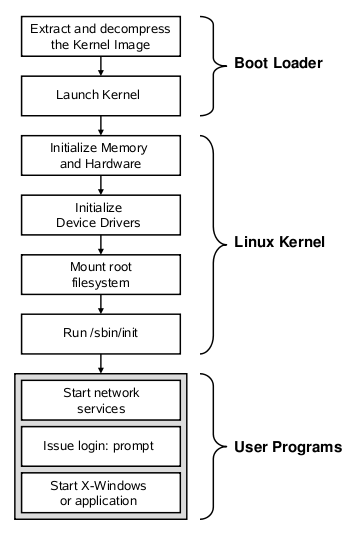
\epsfig{file=figures/Fig_6_2_Boot,width=0.4\textwidth}\\
	  \caption{Boot Procedure}
     \end{center}
\end{figure}
\os{\newpage}

\item[{\rot\bf Scalable behaviour of embedded Linux}]~\\[-3ex]
\bi
	\ite building of a new image (binaries of embedded Linux systems) starts with a configuration part.
	\ite first part is the selection of the ``vendor''.
	\ite specification of hardware details of the development kit (RAM addresses, ROM addresses).
	\ite the next step is the configuration of necessary modules and drivers.

\ei

\os{\newpage}
\begin{figure}[!hbtp]
     \begin{center}
	  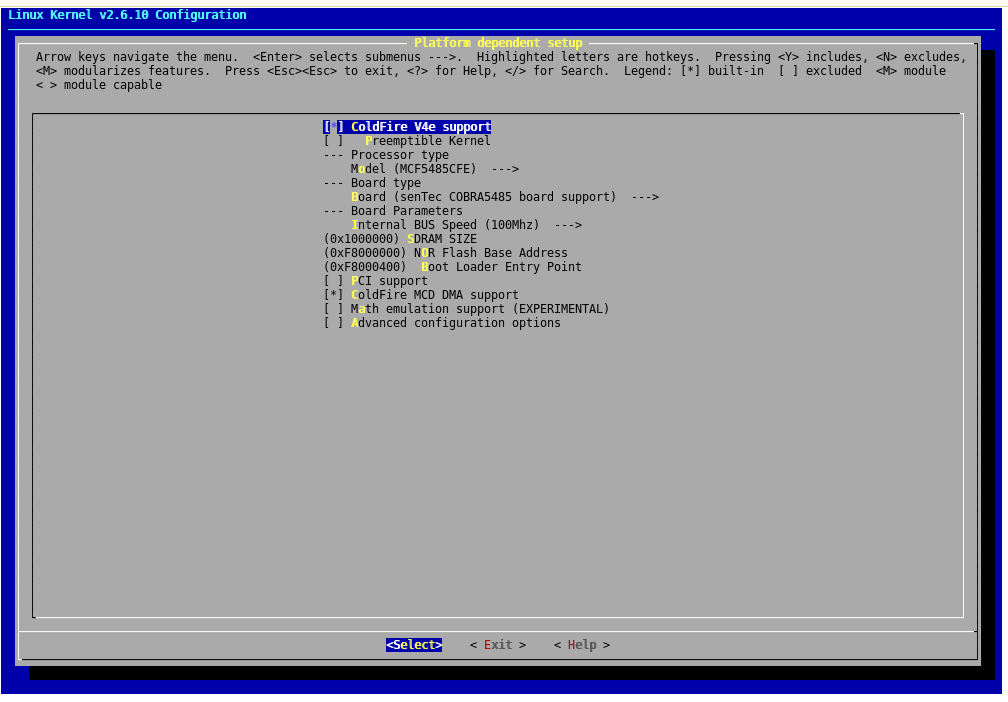
\epsfig{file=figures/Fig_6_3_Vendor,width=0.8\textwidth}\\
	  \caption{Specification of Hardware Details}
     \end{center}
\end{figure}
\os{\newpage}
\begin{figure}[!hbtp]
     \begin{center}
	  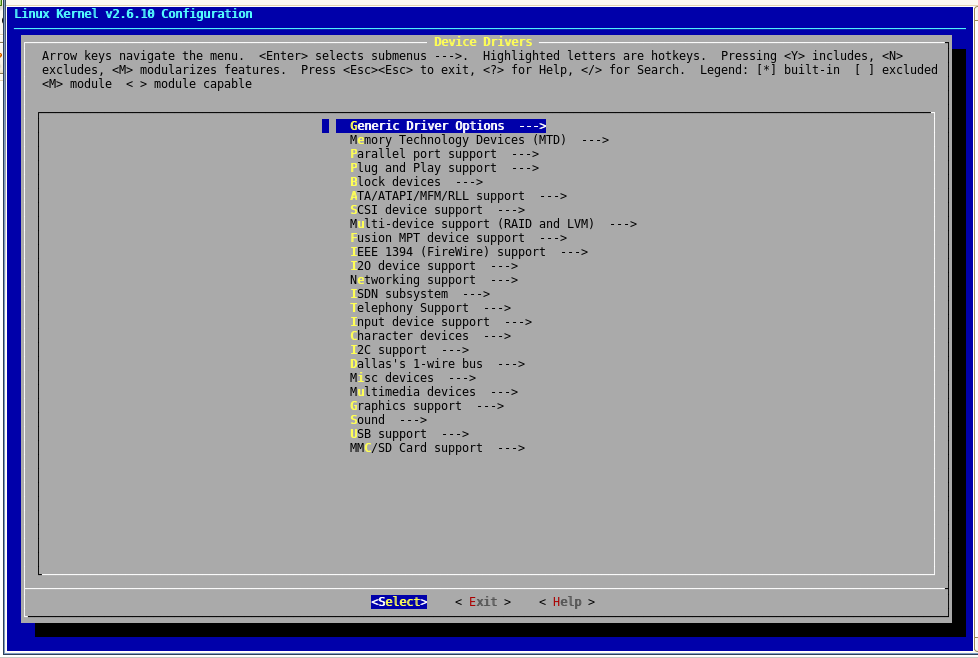
\epsfig{file=figures/Fig_6_4_Drivers,width=0.8\textwidth}\\
	  \caption{Configuration through a Selection of Moduls or Drivers}
     \end{center}
\end{figure}
\os{\newpage}

\item[{\rot\bf Build procedure}]~\\[-3ex]
\bi
	\ite after the configuration (make menuconfig)
	\bi
		\ite start the build process with ``make dep''.
		\ite  and ``make''.
	\ei
	\bigskip
	\ite the Kernel-compilation need a special compiler (gcc-version for the ARM-Processor) und a special binutils (as, ld objtools for the ARM-Processor).
	\ite the result of the Kernel-compilation is a image which is available in two versions.
	\bi
		\ite file ``linux.bin or Kernel.img'' .
		\bi
			\ite a loadable image.
			\ite could be downloaded (serial or usb-interface, needs a monitor program on the target side ).
			\ite execute after a poweron reset or with a jump on a specific address (monitor function).
			\ite useful for test of a configuration.
		\ei
		\bigskip
		\ite file ``romfs''
		\bi
  			\ite a image which could be loaded in the FlashEPROM.
			\ite need a ``Flash''-load program like CF-Flasher.
			\ite embedded Linux starts after the next reset or power-on-reset with the mentioned boot sequence.
		\ei
	\ei
\ei

\item[{\rot\bf Working with embedded Linux in the target}]~\\[-3ex]

\bi
	\ite establish a serial communication link between the target and the PC.
	\bi
		\ite works as standard input/output (stdio) for messages from embedded Linux.
		\ite on the PC-side, a terminal program like ``minicom''  for Linux or ''Hyperterminal'' for Windows is useful.
	\ei
\ei
\os{\newpage}
\begin{figure}[!hbtp]
     \begin{center}
	  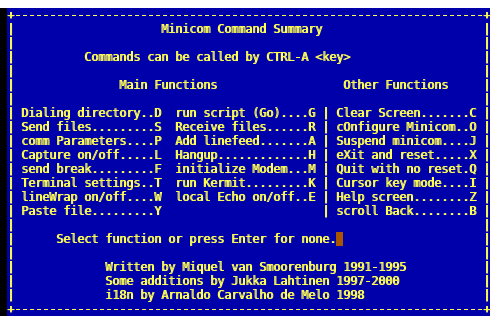
\epsfig{file=figures/Fig_6_5_Minicom,width=0.8\textwidth}\\
	  \caption{Serial Communication Tool Minicom}
     \end{center}
\end{figure}

\os{\newpage}
\begin{figure}[!hbtp]
     \begin{center}
	  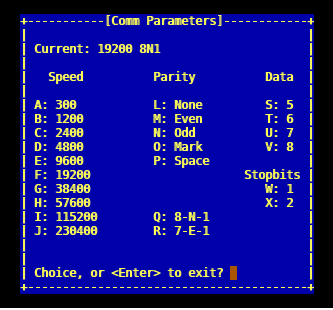
\epsfig{file=figures/Fig_6_5_Minicom_P,width=0.6\textwidth}\\
	  \caption{Configuration of Minicom}
     \end{center}
\end{figure}

\os{\newpage}
\bi
	\ite if an ethernet link is established
	\bi
	  \ite generate a remote connection (via ssh)
	  \bi
	    \ite execution of commandline instructions on the target
	  \ei
	  \ite mount PC partition by NFS
	  \bi
	    \ite target-filesystem can be mounted in the development-filesystem
	    \ite execute programs on the development-side and on the target-side
	  \ei
	\ei
\ei
\begin{figure}[!hbtp]
     \begin{center}
	  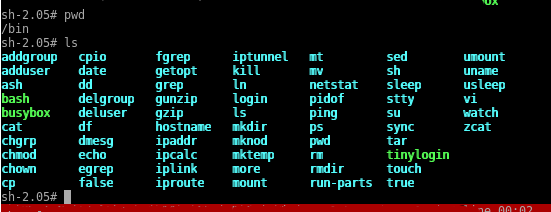
\epsfig{file=figures/Fig_6_6_uCLinux,width=0.9\textwidth}\\
	  \caption{Standard Commandline Interface on the Target-side}
     \end{center}
\end{figure}

\os{\newpage}
\item[{\rot\bf Restrictions when using non VM-systems}]~\\[-3ex]
\bigskip
\bi
	\ite ARM-Processors could operate with a VM (virtual memory) and a non VM System.
	\ite in the case of working without a VM-System:
	\bi
		\ite a user program has full access to the whole memory space.
		\ite as a result, no segmentation fault is possible.
		\ite no dynamic heap \pr instead uCLinux uses a global memory pool (kernel free memory pool).
		\ite no obvious implementation of malloc due to lack of heap.
		\ite no fork sytem call \pr an implementation of ``copy on write'' strategy isn't possible (an alternative is the old BSD vfork and all its limits).
	\ei
\ei
\end{description}

%%%%%%%%%%%%%%%%%%%%%%%%%%%%%%%%%%%%%%%%%%%%%%%%%%%%%%%%%%%%%%%%%%%%%%%%%%%
\section{Cross Compilation}
%%%%%%%%%%%%%%%%%%%%%%%%%%%%%%%%%%%%%%%%%%%%%%%%%%%%%%%%%%%%%%%%%%%%%%%%%%%
\bi
	\ite cross compilation is widely used for programming in embedded systems.
	\ite the programs are written, linked and simulated on a PC (for example) for an embedded system.
	\ite then these executable programs have to be downloaded and started on the target under the control of a monitor program (mostly with a serial connection between the PC and the target).
	\ite after the test in the target the executable program could be stored in the EPROM and executed without a monitoring program
\ei
\os{\newpage}
\begin{figure}[!hbtp]
     \begin{center}
	  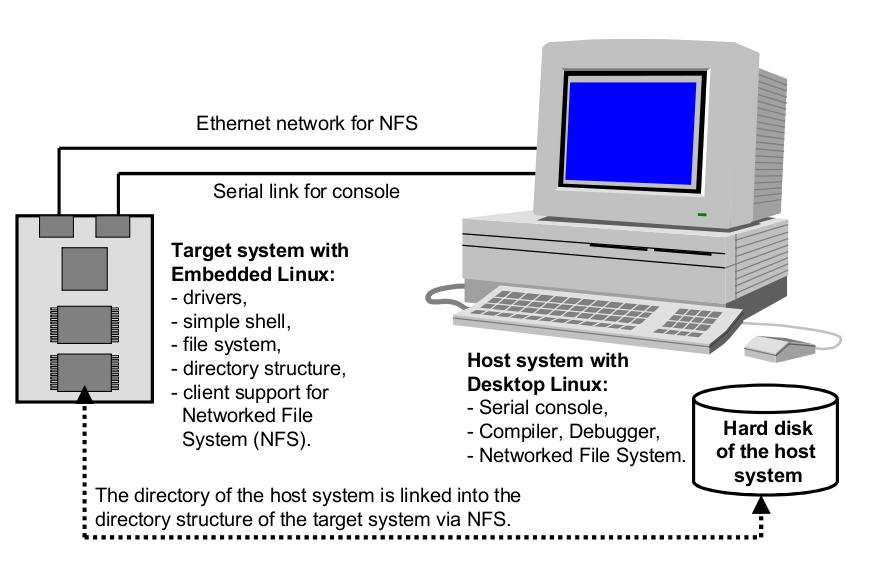
\epsfig{file=figures/Fig_6_7_CrossCompilation,width=0.9\textwidth}\\
	  \caption{Cross Compilation}
     \end{center}
\end{figure}

\os{\newpage}
\begin{description}
\item [{\rot\bf Cross compilation with embedded Linux}]~\\[-3ex]
\bigskip
\bi
	\ite in embedded Linux systems the cross compilation is done for the same reasons as for a standard system.
	\ite the advantage in this case is that the same debugging tools that are available for the test on the PC are also available on tests on the target system (remote debugging).
	\bigskip
	\ite to compile a program for the ARM-Processor a specific toolchain is necessary
	\ite the same toolchain is also used to build the embedded Linux System for the target.
	\ite to generate all parts of the toolchain the standard C-compiler and C-libraries are also involved:
\ei
\os{\newpage}
\begin{center}
 \begin{tabular}{|l|l|}
\hline
Tool & Description\\
\hline
arm-linux-gcc & C-Compiler for ARM-Processor\\
\hline
arm-linux-as & Assembler for ARM-Processor\\
\hline
arm-linux-ld & Linker for ARM-Processor\\
\hline
\hline
arm-linux-ar & Archiver, tool to build, extract and show the contents \\  & of libraries \\
\hline
arm-linux-nm & extracts the symbols of an executable file\\
\hline
arm-linux-objdump & extract the contents of an executable file \\
 & (e.g. disassemble files)\\
\hline
arm-linux-objcopy & tool to generate loadable files from \\
 & the output of the linker (e.g. ``x.bin'' or ``x.ihex'') \\
\hline
 \end{tabular}
\end{center}
\os{\newpage}
\item [{\rot\bf Executable files}]~\\[-3ex]	
\bigskip
\bi
	\ite standard output of the linker (``x.elf'') isn't downloadable.
	\bi
		\ite this file needs a VM-System for loading and execution.
	\ei
	\bigskip
	\ite instead of ``x.elf'' the tool arm-linux-objcopy generates a ``x.bin'' and/or ``x.ihex''-file.
	\bi
		\ite both files are directly downloadable and don't need a VM-System for execution.
		\ite this means both file are linked on an absolute address.
		\ite the ``x.bin''-format is a binary format (could not be read with an editor).
		\ite the ``x.ihex''.format is a text format which is readable with any standard editor.
	\ei
\ei
\os{\newpage}
\begin{figure}[!hbtp]
     \begin{center}
	  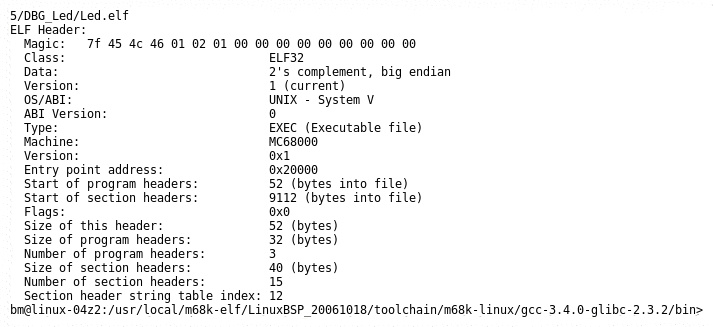
\epsfig{file=figures/Fig_6_8_Info_ELF,width=0.9\textwidth}\\
	  \caption{Information in a ``x.elf''-file}
     \end{center}
\end{figure}



\end{description}
%%%%%%%%%%%%%%%%%%%%%%%%%%%%%%%%%%%%%%%%%%%%%%%%%%%%%%%%%%%%%%%%%%%%%%%%%%%
\section{User Programming in uCLinux}
%%%%%%%%%%%%%%%%%%%%%%%%%%%%%%%%%%%%%%%%%%%%%%%%%%%%%%%%%%%%%%%%%%%%%%%%%%%	
\bi
	\ite user programming implies that a program runs in the user mode of the ARM-Processor.
	\ite if the VM-System is activated \pr the user doesn't have an access to an absolute memory address.
	\bi
		\ite especially a direct access to the registers of interfaces isn't allowed.
	\ei
	\bigskip
	\ite the restrictions imply also that an access to R-, S-, D-registers, CPSR and etc. are not allowed.
	\ite these access could only be done in the supervisor mode (kernel program).
\ei
\bigskip
\bi
	\ite Development of program should be done in tree steps:
	\bi
           \ite first try to generate a program with a cross-compilation for the target, load and then test it.
	      \ite then merge the program together with an image of the operating system and load it.
	      \ite lastly, if necessary implement a "autoexec" function in the init process of the embedded Linux.
      \ei
\ei
\begin{description}
\item[{\rot\bf Cross-compilation with embedded Linux}]~\\
\bi
	\ite the cross-compilation with embedded Linux has the same procedure as the standard cross-compilation for ARM-Processors.
	\ite in preparation for the next two steps it is helpful to use a separate directory which holds all the necessary files (C-files, Header-files, makefile).
	\ite put this directory in the ARM-Linux-file-system '/armLinux/user/' .
	\ite after the compilation mount the directory with NFS in the uCLinux for the target and execute and test the program.
\ei
\bigskip
\item[{\rot\bf Download together with an image of  embedded Linux}]~\\
\bi
	\ite the second step is to integrate the program in an image of uCLinux.
	\ite additional to the cross-compilation, the program also has to be integrated in the build procedure of uCLinux.
	\bi
		\ite the ``central''-makefile for building all the user applications \\ (/armLinux/user/makefile) should expanded with an instruction like:
		\\ \begin{tabular}{l l l l}
		    DIRSc\$(CONFIG\_USER\_CAN)& += & can4linux & (present line)\\
		    DIRSc\$(CONFIG\_USER\_PROGRAM)& += & program & (new line)\\
		   \end{tabular}
		\ite to make the program visible in configuration tool (make menuconfig) of armLinux the file 'config.in' (/armLinux/user/config.in) should expand by:
		\\ \begin{tabular}{l l l}
		    bool 'can4linux' & CONFIG\_USER\_CAN & (present line) \\
		    bool 'program' & CONFIG\_USER\_PROGRAM & (new line) \\
		   \end{tabular}
		\ite to get some more information about the program and how somebody can do the configuration the file Configure.help \\
		(/armLinux/user/Documentation/Configure.help) should expand by
		\\ \begin{tabular}{l l}
		   CONFIG\_USER\_CAN& \\
		    & This package contains some examples\\
		    & using can4linux device driver.\\
		    & \\
		   CONFIG\_USER\_PROGRAM& \\
		    & This programm adds my first functions \\
		    & to uCLinux. I'm not sure whether \\
		    & somebody can use these functions.\\
		   \end{tabular}
		\os{\newpage}
		\ite if in the configuration step, the program is selected, the resulting image contains the program
		\ite to test the image (armLinux) and the program once more, it can be downloaded with the monitor
		\ite the downloaded armLinux (including the program) could be started after a reboot or a reset
	\ei
\os{\newpage}
\ei
\item[{\rot\bf Autostart of a program with embedded Linux}]~\\
\bi
	\ite if the program (which was downloaded together with the armLinux-image) has to be used, the user has to start it.
	\ite embedded Linux offers an automatic start of programs (function of the program init which execute the sript file /etc/inittab).
	\ite the sript-file inittab ask an another skript-file rcS (placed in /etc/rc.d/rcS) and this file switch over to rc.local (/etc/rc.d/rc.local).
	\ite an auto start could be done by addition in the file rc.local (but this means that the user has to change this file and this is obviously not an autostart, escpecially not for the first time).
	\ite to do a 'real' auto start of the file \\
	/armLinux/defconfigs/vendors/senTec/etc/rc.d/rc.local has to changed and then a new image has to be created.
	\ite when this image is loaded in the FlushEPROM (with the program CFFlusher) then after a reset the program is automatical started without an interaction with the user.
\ei

%\os{\newpage}
%\item[{\rot\bf Applications for ARM Cortex on a BeagleBoard or a Rasberry Pi Board}]~\\
%\begin{center}
%\begin{tabular}{|l|l|}
%\hline
%Exercice 1 & \textbf{BeagleBoard: Digital I/O} \\
%\hline
%Participants & Ramachandran, Mahalinam; Amar, Jadhav \\
%\hline
%Presentation & Mo. 24.6.2013, 16.00 \\
%\hline
%\hline
%Exercice 2 & \textbf{BeagleBoard: Set up an Eclipse-based } \\
%	   & \textbf{Cross Compilation} \\
%\hline
%Participants & Jamshid, Ummattam; Archana, Basavalingappa; \\
%	     & Sharath, Chandra \\
%\hline
%Presentation & Wed. 24.6.2013, 16.15 \\
%\hline
%\hline
%Exercice 3 & \textbf{BeagleBoard: Use  GPIO and a external} \\
%	   & \textbf{D/A-Converter to build a Function Generator} \\
%\hline
%Participants & MD. Arifur Rahman, Neecati, Gouthan \\
%\hline
%Presentation & Wed. 24.6.2013, 16.30 \\
%\hline
%\end{tabular}
%\end{center}



\end{description} 